\documentclass[12pt]{article}

\usepackage{graphics}
\usepackage{epsfig}
\usepackage{times}
\usepackage{amsmath}
\usepackage{booktabs}


\usepackage{hyperref}

% <http://psl.cs.columbia.edu/phdczar/proposal.html>:
%
% The standard departmental thesis proposal format is the following:
%        30 pages
%        12 point type
%        1 inch margins all around = 6.5   inch column
%        (Total:  30 * 6.5   = 195 page-inches)
%
% For letter-size paper: 8.5 in x 11 in
% Latex Origin is 1''/1'', so measurements are relative to this.

\topmargin      0.0in
\headheight     0.0in
\headsep        0.0in
\oddsidemargin  0.0in
\evensidemargin 0.0in
\textheight     9.0in
\textwidth      6.5in

% \title{{\bf Doctoral Thesis Proposal} \\
% \it Thesis proposal}
\title{{\bf Big Location Data: \\ Balancing Profits, Promise, and Perils} \\
\it Thesis Proposal}
\author{ {\bf Chris Riederer}  \\
Department of Computer Science \\
Columbia University\\
{\small mani@cs.columbia.edu}
}
\date{\today}


%%%%%%%%%%%%%%%%%%%%%%%%%%%%%%%%%%%%%%%%
%%%%% COMMANDS
\newcommand{\chap}[1]{Chapter~\ref{#1}}
\newcommand{\fig}[1]{Figure~\ref{#1}}



\begin{document}
\pagestyle{plain}
\pagenumbering{roman}
\maketitle

\pagebreak
\begin{abstract}
% Big data!! Accompanied by risks and benefits
The ``Big Data" era has begun, bringing with it a host of possibilities and concerns.
The ability to store and process records of minute behavioral details about billions of people will hopefully lead to more efficient and effective businesses, governments, and organizations.
At the same time, these new collections of data present societal risks, enabling mass surveillance, a potential loss of privacy, and the capability to computationally discriminate at massive scale.

% Location data, a subset of big data.
A rich subset of this data is human mobility data: records at an individual scale detailing where and when someone moves.
This data is now captured like never before due to the rise of smartphones and other cheap and ubiquitous electronic devices.
This location data can be a boon to both profit centers and scientific understanding, but comes with many risks attached.
The places we visit can reveal much about ourselves, whether proclivities towards particular type of food and hobbies, or more private characteristics of race, religion, sexuality, and political affiliation.
As organizations begin to harness this data, it is clearly important to make sure that such information is used in a way that reduces potential harms to individuals or vulnerable groups.

% Description of completed work and proposal
In this document, I describe recent and in-progress work that attempts to balance the scientific and engineering promises of location data with the potential risks, looking at three classes of problems.
I begin with my work on anonymity, examining when location data retains an identifiable ``fingerprint" of a user that can be linked to data sets generated by completely separate behaviors, making anonymization difficult or impossible.
I continue with work focusing on privacy and economics, aiming to reconcile the economic incentives for firms to collect location data with usable user choice and a better understanding of users' beliefs and desires in relation to data capture.
Next, I examine the relationship between location data and algorithmic bias, showing that location data can be used to infer sensitive traits and developing a tool to inform users about what their data may be revealing.
% I conclude with a proposal to research the algorithmic bias that may be inherent in location-based advertising systems, combining millions of locations collected from social media, computer vision, and the state-of-the-art results in algorithmic de-biasing.

I conclude with my proposal to conduct an analysis that will show the conditions in which a firm may engage in location-based advertising without unfairly distributing their offers across different demographics.
This work will combine a dataset of millions of locations collected from social media, computer vision techniques, and state-of-the-art results in algorithmic de-biasing to show, for the first time, the trade off between revenue and fairness in a location-based advertising setting.

% business - profits
% ngo - effectiveness
% govt - efficient

\end{abstract}

\pagebreak
\tableofcontents
\pagebreak

\cleardoublepage
\pagenumbering{arabic}

\section{Introduction}
\label{ch:intro}
% Ermergerd big data
The era of Big Data has the potential to transform all aspects of society, from business operations to individual leisure time, from medicine to elections.
As the cost of computation and data storage has fallen, and as more human behavior has moved to easily-recorded digital mediums, both public and private institutions have captured and stored more and more information.
``Data is the new oil", analysts have proclaimed, as businesses seek to become more efficient or create innovative digital products. % TODO: cite
``Data will power the cities of tomorrow" governments have proclaimed, releasing their troves of data to the world.

% Shift: what are the problems
The excitement of the potential gains has been tempered by many potential concerns.
% Anonymity: NSA
With the desire for public agencies that could more accurately prioritize safety concerns has come massive surveillance, both by companies and governments, raising concerns of \textbf{anonymity}. % TODO: cite
% Economics: price discrimination
With the belief that Big Data would lower costs and benefit consumers has come evidence of large-scale price discrimination~\cite{wsj, Anonymous:2012wi}, with its impacts possibly most felt by already economically vulnerable populations, raising concerns of \textbf{economics}.
% Algorithmic bias: bail-setting
And with the hopes of making government more fair and efficient have come allegations that seemingly impartial algorithms actually encode unfair racial biases~\cite{propublica:bias}, raising concerns of \textbf{algorithmic bias}.
We must carefully consider how to obtain the benefits of the Big Data Age without paying too high a price.

% Location data
% Although Big Data encompasses the massive colletion of information from all areas of human activity, of particular interest and concern is data generated by the everyday activity of human beings, as this 
One particularly interesting and sensitive subset of Big Data is information relating to the real world movements of individuals: ``location data".
As this data is tied to actual physical movements, it is of enormous interests to businesses and governments.
When people move, they are expending energy and money to do so, as opposed to the many relatively low-cost digital behaviors captured online.
Thus, location data provides a valuable input for many problems, as evidenced by academic proof-of-concepts and by the many businesses and services surrounding it's capture, such as Google Location Services, Foursquare\footnote{\url{foursquare.com}}, Placed\footnote{\url{placed.com/}}, and many more.

% Problem: how to use location data safely?
% TODO: explain a bit more about what this case was about?
Along with its valuable signal again comes concerns of safety and privacy.
In the United States v. Jones decision, in which the Supreme Court wrestled with the legality of law-enforcement placing a GPS tracker on a car without a warrant, Justice Sotomayor wrote 
``disclosed in [GPS] data ... [are] trips the indisputably private nature of which takes little imagination to conjure: trips to the psychiatrist, the plastic surgeon, the abortion clinic, the AIDS treatment center, the strip club, the criminal defense attorney, the by-the-hour motel, the union meeting, the mosque, synagogue or church, the gay bar and on and on"~\cite{jones2012us}.
Clearly, if location data is to be used by analysts, it must be done so in a way that is extremely careful and respectful of user preferences.
% TODO: add another sentence

In this thesis proposal, I examine work that attempts to reconcile the benefits of data-mining location data with three key areas of concern: anonymity, economics, and algorithmic bias.
I will begin with a background section which introduces the core concepts found in this proposal, continue with several chapters relating to the afore-mentioned areas of concern, and conclude with a final discussion of next steps in making big location data safe and fair to use.

\subsection{Anonymity}
% Linking Users Across Domains with Location Data
% FindYou
\chap{sec:anon} examines the possibility of anonymizing location data. %TODO: edit
Prior work has shown that users are highly unique in their location patterns, leaving them vulnerable to deanonymization (see~\ref{ssec:privacy}).
Here we take this a step further, showing not only that this vulnerability exists, but that users indeed can be linked to other datasets.
Additionally, we provide a tool to users that aggregates and displays their location data along with the potential inferences made from it.

\subsection{Economics}
\chap{sec:econ} focuses on location data, privacy, and economics. %TODO: edit
We begin with work that seeks to understand user attitudes to their privacy and the economic value of their information.
Specifically, it examines an alternative to the current practice of firms offering free services in exchange for full control over user data.
The alternative model is one in which users control their data and make decisions about when to sell access to their info, and to whom.


\subsection{Algorithmic Bias}
% I Don’t Have a Photograph But You Can Have My Footprints
% Under submission work on demographic labeling
% Current work on bias!
\chap{sec:bias} shows the potential for location data to be part of systems that %TODO: edit
We gather a dataset of locations attached to demographic information from a popular image-sharing mobile application.
This data allows us to study the differences in human mobility across different groups, and moreover, to show that demographics can be inferred using only location data.
This raises questions about the sensitivity of location data, and about the potential for bias in systems that make decisions based on location data.
We examine other methodologies for inferring demographics from social network data and discuss debiasing of algorithms.

\chap{sec:proposal-i}

\chap{sec:proposal-ii}

I conclude with a plan for completing this work in \chap{sec:plan}.




\section{Background}
\label{sec:background}
% \subsection{Location Data}
\textbf{What is location data?}
Most generally, location data is information relating people to places.
Typically, this relation is the fact that a person was at a place.
Adding time into the figure, the relation could be that a person was at a place at a particular time.
However, location data could also include relations about the importance of a place in someones life, such as them living in a location, working at a location, or having spent a quantity of time in a location.
Though location data does not need to be associated with user IDs, in this work we will consider that there is always attached some sort of user ID that uniquely identifies the user in the dataset, possibly de-personalized.

Location data can be described in two main ways: \textbf{geographically} or \textbf{semantically}.
\emph{Geographic} data can be described by a latitude-longitude data on the globe.
\emph{Semantic} location data refers to an identifier used within that dataset.
This could have some information available to a common user, e.g. ``New York City", or it could simply be an identifier, e.g. 7.
Note that often these two may be combined or used together.
A location such as ``CEPSR Office 618, Columbia University" (the author's office) indicates a very small, non-ambiguous location that can easily be mapped to geographic coordinates.
Semantic location data can sometimes present a privacy problem, as an association with a place could indicate sensitive attributes, such as someone's religion, political affiliation, health, or sexuality.
In this work, I will typically assume location data is also tagged with temporal data, and I will use the terms location data and spatiotemporal data interchangeably.

To put this more formally, we can define a single data point $p$ of location data to be:
\[ p = \langle u, l \rangle \]
or, including time:
\[ p = \langle u, l, t \rangle \]
where $u$ uniquely identifies a user, $l$ uniquely identifies a location, and $t$ specifies a time.
Note that $l$ could be a latitude-longitude pair in the geographic case or an ID in the semantic case.

\textbf{How is location data collected?}
Location data can be captured passively or actively.
\textbf{Actively captured} location data is only recorded when the user takes some action.
Note that this action does not need to inherently be ``about" location data, for example, a user making a call from a cell phone or swiping a credit card is typically not consciously thinking about their location data. 
A record of their location is created as a by-product of their use of that technology.
\textbf{Passively captured} is meant in a stronger way-- the user's location is captured without the user making any kind of action.
This can occur through tracking apps.
An example is MapMyRun\footnote{\url{http://www.mapmyrun.com/}}, an app where users record their routes while running, in order to track distance and progress in meeting exercise goals.
Although the user took an action to start recording their location, the location is recorded in the background with no user action from then on, and hence we call it ``passive".
Another example is Google's location history.
Google records location data in the background of a users Android phone every few minutes.
A map of everywhere a user (with an Android phone with location history turned on) is available at \footnote{\url{https://www.google.co.in/maps/timeline}}.

% \textbf{What is location used for?}
% TODO



% \subsection{Privacy}
% \label{ssec:privacy}
% Privacy has been an important concept, brought to the forefront of public debate as surveillance of users has grown, both by governments and private companies.

% ADD MORE STUFF

% In this work, we will focus on two technical conceptions of privacy, \emph{k-anonymity} and \emph{differential privacy}.

% \textbf{k-anonymity} 

% \textbf{Differential privacy}


% \subsection{Bias}

% \subsection{Online Advertising}



\section{Location Data, Privacy, and Economics}
\label{sec:econ}
% Introduction

% The primary goal of big data is to guide decision making.
The online economy is based primarily on advertising.
The income of a firm roughly translates to (number of impressions) x (dollars per impression).
I am trying to keep this abstract and not saying that firms are always getting paid for impressions, as other models like paying per click or per sale or other action are quite common.
Really the argument here is that firms make money based on how many people come to their site and how well they can target advertisements to those individuals.
This gives firms an incentive to gather as much information about their users as possible so that they can better target ads to them.

% sec:background
% This can of course present a privacy issue.
This framework presents a challenge to privacy.
User information is collected and gathered in one centralized place.
There are multiple risks involved here: the firms themselves may use the information in ways the users disagree with, the firms may sell or be coerced to give their information to other firms or governments, or the firms may fall victim to cybersecurity attacks, leaking information to other sources.
TODO: cite some stuff.

As ways to counter this, schemes have been proposed to encrypt user behavior and information, denying all access to a firm.
However, this would deny firms the ability to make money, meaning no services would be provided for users and possibly a lower global utilty be reached.
Thus, schemes that ignore this economy however are unlikely to be adopted.
Companies need to make money to function.
Currently, users seem happy to provide their data in exchange for free services.
A concern is that users do not have a good idea of their data and do not know how it is being used and to whom it is accessible.

Therefore it is important to gain an understanding of how users value their information, what they believe firms are doing with their data, and what users are comfortable with in terms of data use.


\subsection{Related Work}


\subsection{Completed Work}

How does one determine how a study participant values something as abstract as 
In our work, ``Your Browsing Behavior for a Big Mac", TODO(cite) we utilized 
% As demonstrated 

\begin{itemize}
  \item Your Browsing Behavior for a Big Mac (maybe?)
  \item For Sale: Your Data. By: You (some portion?)
  \item Challenges of Keyword-Based Location Disclosure
\end{itemize}

``Your Browsing Behavior for a Big Mac"
User privacy is extremely important.
However, there does not exist a strong understanding of how users value their privacy.







\section{Location Data and Anonymity}
\label{sec:anon}




\subsection{Related Work}
\begin{figure}[t]
  \centering
  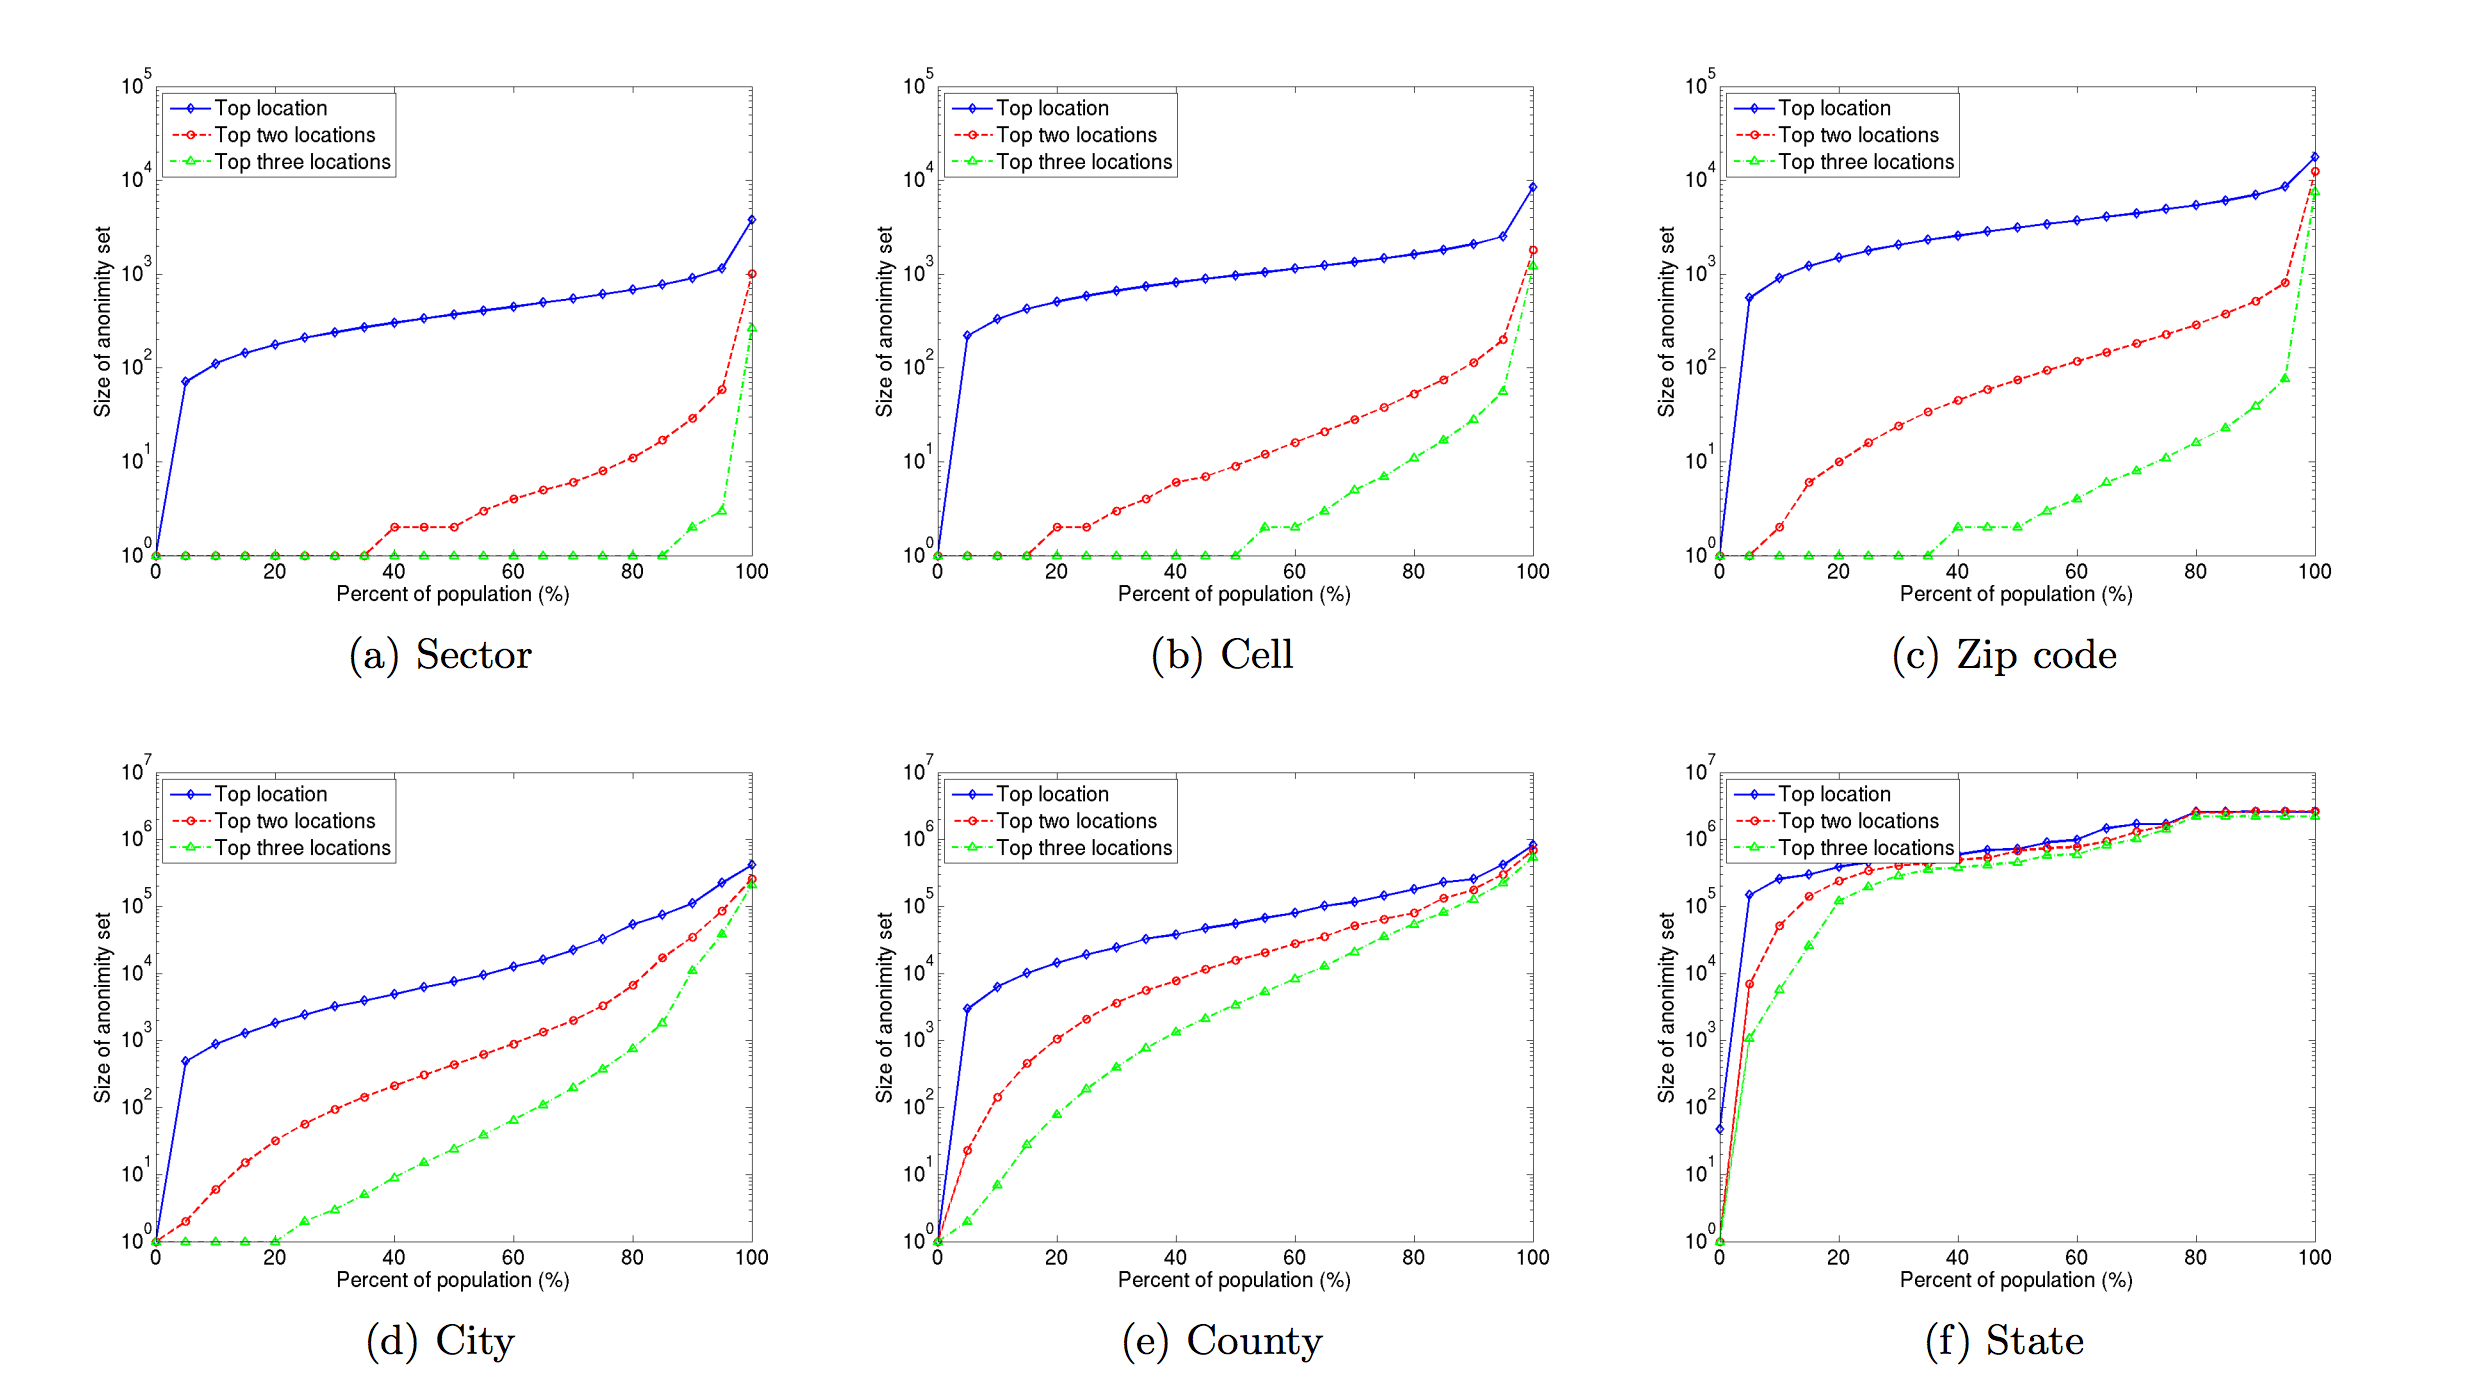
\includegraphics[width=\linewidth]{fig/zang_bolot.png}
  \caption{Figure from~\cite{Zang:2011hk} depicting the size of anonymity sets for top $n$ most visited location of users.
           Locations are varied in granularity, from cell sectors to US states.}
  \label{fig:zang_bolot}
\end{figure}

Location data for individuals is highly unique and thus difficult to anonymize.
The first large-scale study of the $k$-anonymity of location data was appropriately titled ``Anonymization of Location Data Does Not Work"~\cite{Zang:2011hk}.
The paper used data from cell phone call detail records (or CDR, see~\chap{sec:background}) for 25 million United States users over a 3 month period.
The authors represents each user as simply their top $n$ most visited locations, varying $n$ from 1 to 3.
Additionally, the authors varied the granularity of the locations, with the smallest as cell sector and the largest as state.
Remarkably, using 3 locations at a cell level made half of all users completely unique, and 3 locations a sector level made 85\% of all users unique.
A figure detailing this result and results for other granularities and values of $n$ is depicted in~\fig{fig:zang_bolot}.
The authors went on to analyze the impact of geography (comparing different states and cities), mobility (distances between top locations), and social networks on anonymity.


The Montjoye nature report


\subsection{Completed Work}
% Completed work introduction
I have investigated the anonymity of location data for users

\subsubsection{Linking Users Across Domains with Location Data}
% Background...
Although prior work showed location to be highly \emph{unique} and thus posibly \emph{vulnerable} to de-anonymization, no data was actually de-anonymized in practice.
Indeed, just because a data source is highly unique does not mean it can be de-anonymized.
For example, much of cryptography relies on creating highly unique but unpredictable sequences of numbers.
To put it more concretely, imagine that each individual had a die with 1000 sides, and each side represented a location.
If, quite hypothetically, humans decided where to go next by rolling this die, their movements would look very unique.
However, since the movements are random and unpredictable, my movements from different time periods will be indistinguishable from those of a different individual.

TODO: put some math here?

Another possibile break in the argument that uniqueness implies vulnerability is the important factor of sampling.
The datasets dealt with here (phone records, social media posts) are all \emph{actively} collected: each data point exists if and only if the user has taken an action.
Intuitively, the location data from different sampling data sources should look very different.
An individual may be more likely to make phone calls in quiet places, like the home or office, and take geotagged location photos in popular tourist destinations or restaurants.

TODO: put some math here?

In ``Linking Users Across Domains with Location Data", published at WWW in 2016~\cite{riederer2016linking}, we tackled this problem, linking users across two entirely different datasets.

% Describe problem setting
\begin{figure*}[t]
  \begin{center}
    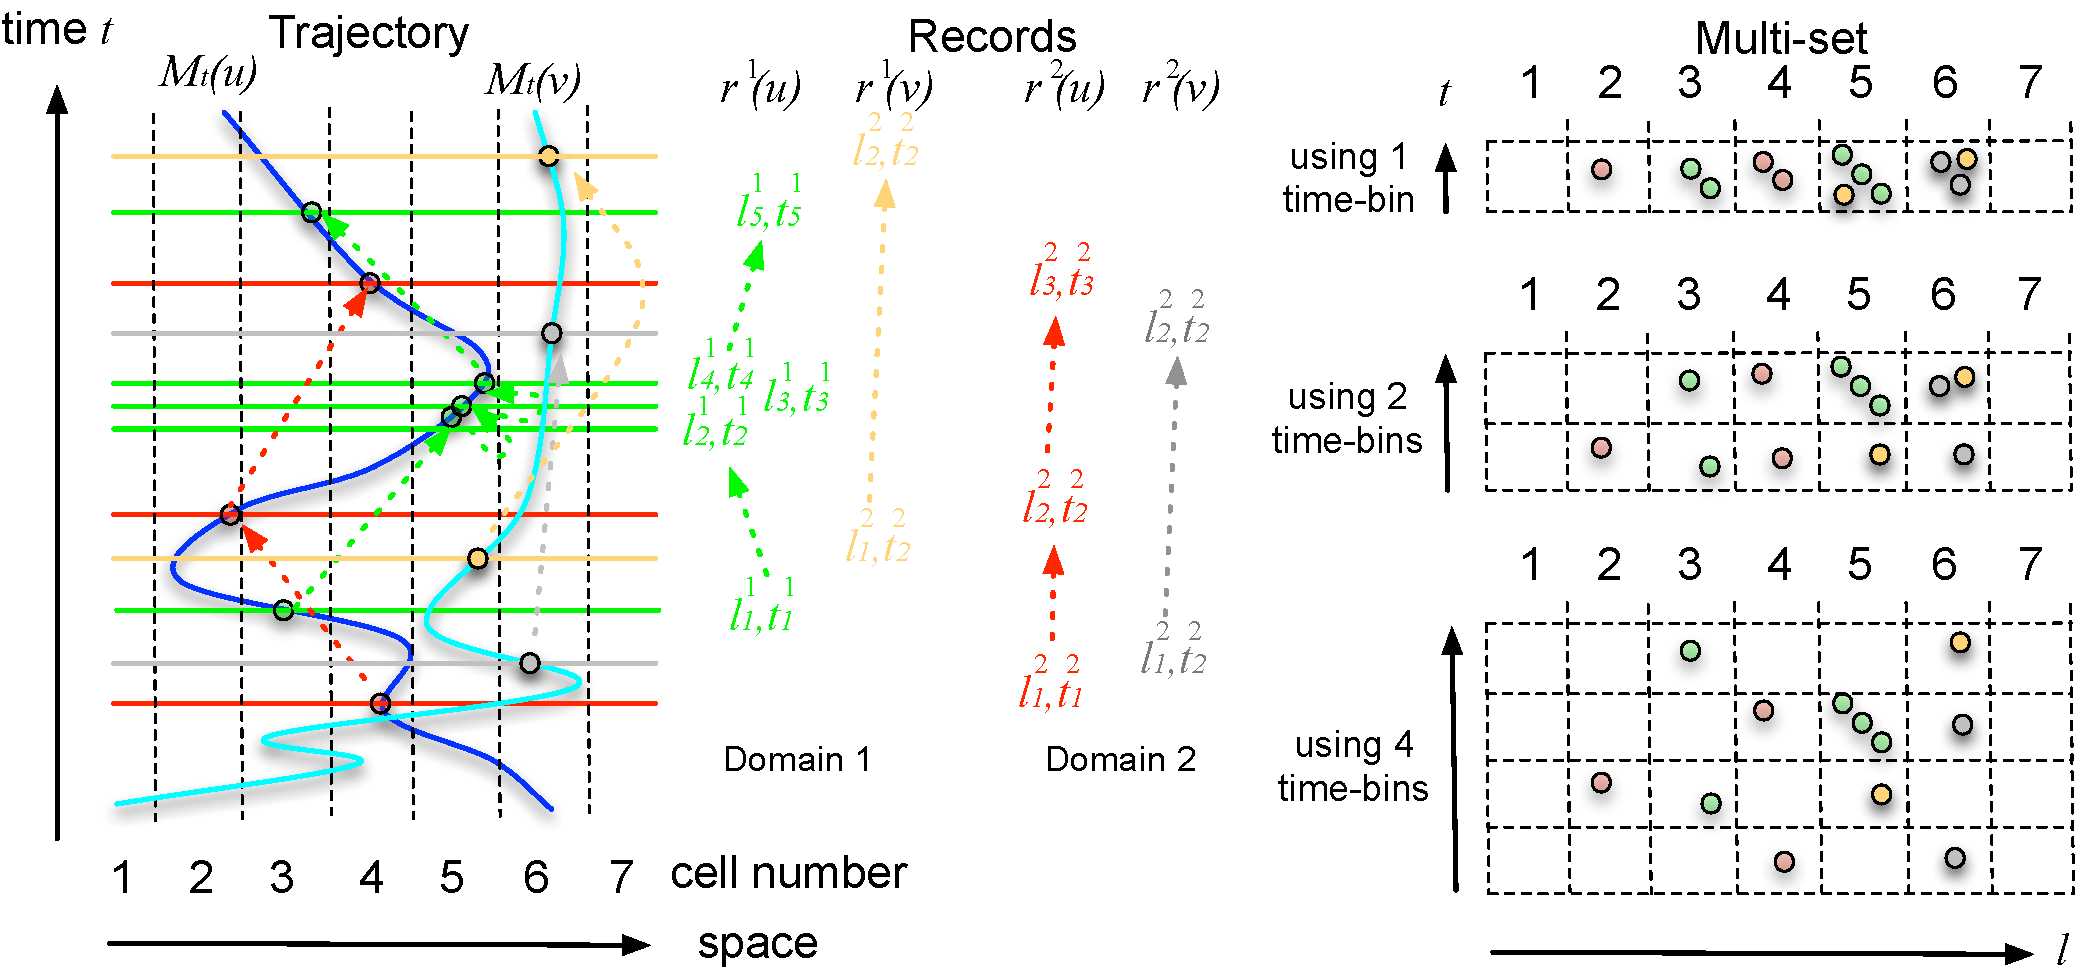
\includegraphics[width=0.65\linewidth]{fig/linking_explain.pdf}
  \end{center}
  \caption{Two space-time trajectories with associated footprints in two domains.}
  \label{fig:linking_explain}
\end{figure*}

% Describe problem
We formalized the problem in the following manner.
We defined $U$ and $V$ to be sets of $n$ user accounts in two separate domains.
Each account is a itself a set of spatiotemporal points $p$, where
\[ p = \langle u, l, t \rangle \]
with $u$ being a user ID unique to either $U$ or $V$, $l$ is a location, and $t$ is a time.
We denoted $\sigma_I$ to be a true (``identity'') mapping that correctly links the two accounts of the each user across $U$ and $V$.
The goal then, of this work, is to recover $\sigma_I$.
    
We made a series of simple assumptions about human mobility.
We broke time into discrete ``bins" of a certain length, and then declared the number of checkins a user has at each location in time bin to be Poisson distributed according to a rate paramater $\lambda$ unique to that time and place.
This is a simple but reasonable assumption, and Poisson distributions are often used to model rare events (like checkins).

This model generates the \emph{real world} mobility of a user.
We assume that this real world mobility is sampled independentally and randomly for the two different data sets with probability $p_U$ and $p_V$.

\fig{fig:linking_explain} provides a visual illustration.
On the left side of the image are two real world trajectories, denoted with a blue and turquoise line.
The x axis shows space and the y axis shows time.
The colored circles (red, green, gray and yellow) show times and places where the real world trajectories are sampled, with (for example) a geolocated photograph, phone call, or checkin.
The challenge is that we only see the green, yellow, red, and gray trajectories in the middle of the image, and we must figure out the true association across datasets.
In this example, red should go with green and gray with yellow.
On the right side of the image, the concept of time bins are illustrated.
We discretize time with varying sized time bins.
The top uses one large time bin, essentially ignoring time, whereas the bottom breaks time into four sections, essentially saying two locations are only the same if the checkins occur near one another in time.

% Describe algorithm
% Based on these assumptions, we were able to develop a maximum likelihood 

% Describe dataset
\begin{table*}
  \centering
  \begin{tabular}{llrrrrr}
    % \toprule
            &        & Number & Number  &   Median  &  Number   &           \\
    Dataset & Domain & Users & Checkins &  Checkins & Locations & Date Range\\
    \midrule
    FSQ-TWT   & Foursquare  & 862 & 13,177  & 8    & 11,265 & 2006-10 -- 2012-11 \\
              & Twitter     & 862 & 174,618 & 60.5 & 75,005 & 2008-10 -- 2012-11 \\
    \addlinespace
    IG-TWT    & Instagram   & 1717 & 337,934 & 93 & 177,430 & 2010-10 -- 2013-09 \\
              & Twitter     & 1717 & 447,366 & 89 & 182,409 & 2010-09 -- 2015-04 \\
    \addlinespace
    Call-Bank & Phone Calls       & 452 & $\sim$200k & $\sim$550 & $\sim$3500 & 2013-04 -- 2013-07 \\
              & Card Transactions & 452 & $\sim$40k & $\sim$60 & $\sim$3500 & 2013-04 -- 2013-07 \\
    % \bottomrule
  \end{tabular}
  \caption{Overview of datasets used in study. For FSQ-TWT and IG-TWT, number of locations refers to locations at a 4 decimal GPS granularity (position within roughly 10m).}
  \label{tab:link-data}
\end{table*}

We evaluated this algorithm on multiple real-world datasets.
Gathering the data in itself was a significant challenge, as each dataset needed to contain individuals with identities linked across two different data sources.
Collecting information from one data source is enough of a challenge by itself, given unexpected and changing data formats, connectivity problems, rate limits, and more.
Getting ground truth data across two datasets is thus more difficult, as two APIs need to be dealt with and user identities must be verified across the two.

We gathered three datasets:
\begin{itemize}
  % Data from foursquare checkins and geolocated tweets, from another paper.
  \item \textbf{Foursquare-Twitter} (FSQ-TWT): 
  checkin data from the location-based social networking and review site Foursquare \footnote{\url{https://foursquare.com/}} and geotagged updates from the microblogging site Twitter \footnote{\url{twitter.com}}. 
  This data was obtained in a prior work by other authors who allowed us to use their data~\cite{Zhang:2014ij}.
  We expect the behavior to be somewhat different across the two networks; Foursquare is primarily used to review restaurants, and Twitter is generally used.

  % Geolocated photos and geolocated tweets. Not the exact same. Got twitter account from profile. Medium difficulty.
  \item \textbf{Instagram-Twitter} (IG-TWT):
  Geolocated photographs from the image sharing site Instagram \footnote{\url{instagram.com}} and geotagged updates from the microblogging site Twitter.
  We first crawled Instagram, and then found users who had posted their Twitter usernames in their profiles.
  For each of these users, we used Twitter's API to crawl their public tweets.
  We expected this dataset to be the easiest to link, as there were high numbers of checkins on both sites for most users.

  % Cell phone calls (located to cell tower) and geocoded businesses.
  \item \textbf{Cell phone-Credit Card} (Call-Bank):
  Phone calls associated with geolocated cell towers (CDR) and credit or debit card transaction data associated with geocoded businesses, all from one G20 country.
  Locations were declared the same if the lat-lon of business was within a cell created via a Voronoi tesselation.
  This data was very sparse and the behaviors generating data seems to be very different in the two sets, making us hypothesize that we would have our worst results on it.
\end{itemize}

Statistics about these datasets is summarized in Table~\ref{tab:link-data}.

% Describe results
\begin{figure*}[th!]
  \centering
  \hspace{-0.7cm}
  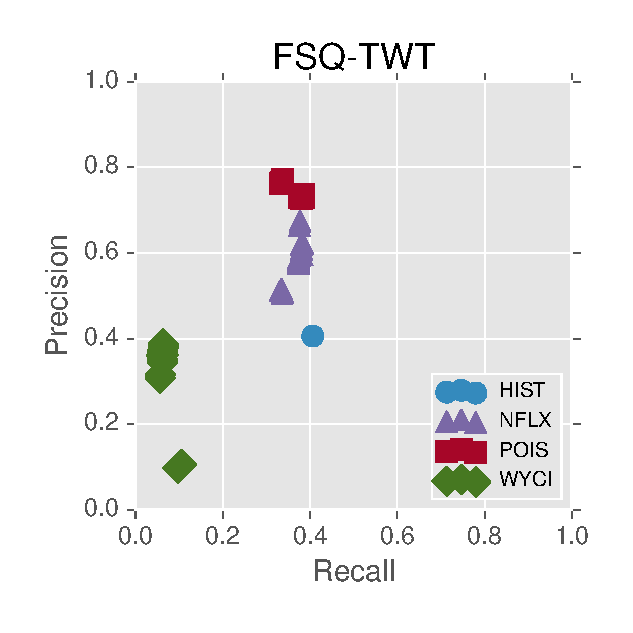
\includegraphics[width=0.35\linewidth]{fig/fs_scatter.eps}
  \hspace{-0.7cm}
  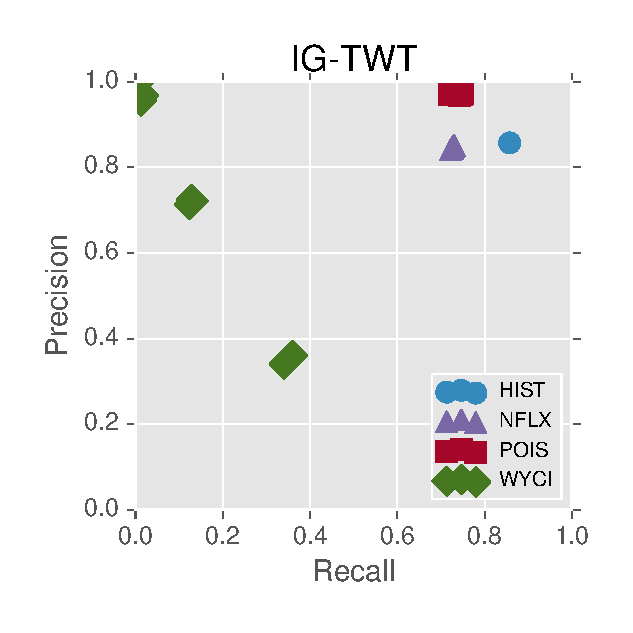
\includegraphics[width=0.35\linewidth]{fig/ig_scatter.eps}
  \hspace{-0.7cm}
  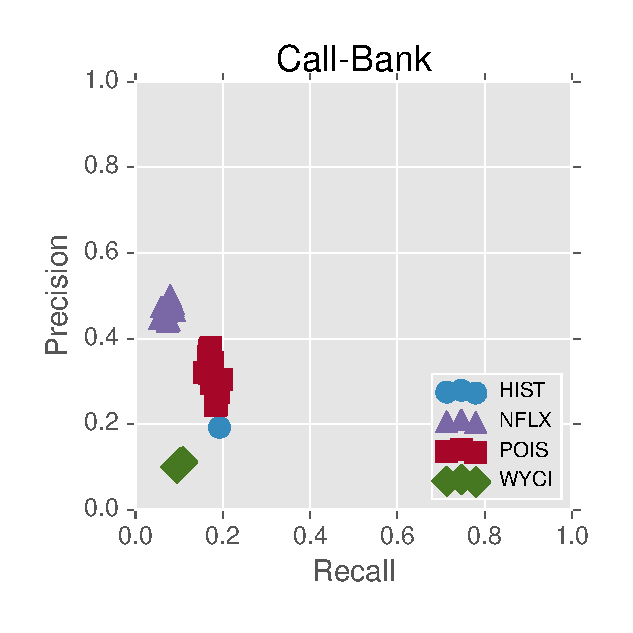
\includegraphics[width=0.35\linewidth]{fig/gd_scatter.eps}
  \caption{Precision and Recall plots for each dataset.}
  \vspace{1ex}
  \label{fig:link-prec-recall}
\end{figure*}

We now turn our attention to experimental performances of our algorithm. 
In Figure~\ref{fig:link-prec-recall}, we show the precision recall plots for our algorithm (for different eccentricity values) and for the other three reconciliation techniques: HIST, NFLX and WYCI. 
For our algorithm, we used estimated parameters and  for the other techniques, we used optimal parameters (found via exhaustive search).

There are several interesting observations that we can make on Figure~\ref{fig:link-prec-recall}. 
First, on the public dataset FQ-TWT our algorithm outperforms all prior methods (especially in precision). 
Nevertheless it is interesting to note that the precision of all methods is not ideal, probably due to sparsity of the data.

A second interesting observation is that our algorithm achieves very high precision when the dataset is more rich. 
In fact when we then turn our attention to our second dataset, the live service (IG-TWT) that we crawled, we obtain almost perfect precision. 
Note that not all the other techniques, for example NFLX, are able to leverage the denser data, as much.

Finally we test our method on a much more heterogeneous dataset (Call-Bank) that is also more realistic and sensitive. 
In this setting our algorithm outperforms previous techniques, with none of the previous algorithms able to achieve good precision and recall at the same time. 

% TODO(can possible add more results)
Other results found that our algorithms rapidly improved with more data.
Additionally, varying the size of timebins or the eccentricity parameter or number of terms did not have a large impact on results, meaning our algorithm's performance should remain stable to different sets of parameters.

% Conclusion?


\subsubsection{FindYou: A Personal Location Privacy Auditing Tool}




\section{Location Data, Demographics, and Bias}
\label{sec:bias}
% Introduction

\subsection{Related Work}


\subsection{Completed Work}
From countries, states, and regions to neighborhoods, local meeting houses, or churches, the places we live and visit are tightly connected to our identities.
Location information gathered about an individual over time can reveal much more than a home location.
In fact, patterns in human mobility can reveal more private components of an individual's 
blah, such as their race, gender, or economic status.

In this section, I will discuss two works which explore these issues.
Both rely on a dataset connecting images to mobility through geotagged photos on the image-sharing site Instagram.
In the first, we label faces for gender, race, and other attributes, and explore whether these features can be inferred from locations visited.
In the second, we evaluate the use computational vision techniques to scale up the use of Instagram to connect mobility to demographics for an ``automated census".


\subsubsection{I Don’t Have a Photograph But You Can Have My Footprints}

% \section{Introduction}
Human mobility is intimately intertwined with highly personal behaviors and characteristics. 
Previous studies of mobility centered on the risk of either re-identification in sensitive anonymized location datasets or on protecting visits to private locations~\cite{de2013unique,Guha:2012ws}.
However, the re-identification risk based on individual locations is not the only threat. 
% Many users are producing a series of digital footprints, which might be innocuous individually, however, taken together can create a sparse yet informative view allowing inferences from their whereabouts. 
% The benefits of revealing locations are obvious: location data can be used for personalizing recommendations~\cite{ICWSM112886} and displaying more relevant advertising~\cite{Lindamood:2009:IPI:1526709.1526899} in order to finance free online services. However, the downsides are more difficult to assess. While an individual data point may create no privacy risk, an aggregated dataset might enable inferences beyond a user's expectation.
In this section, the full version of which appears in~\cite{riederer2015cosn}, we explore the discriminative power of location data. Solely based on mobility patterns, which we extracted from photosharing network profiles, we infer users' ethnicities and gender both on a demographic and an individual level. This exploration stands in contrast to limitations of previous studies as our paper brings together the following contributions:
\begin{itemize}
  \item We show how photosharing network data can be leveraged to extract mobility patterns using a new method for creating location datasets from publicly available resources. Our method combines the use of online social networks and crowdsourcing platforms. It has the advantage that it generally enables \emph{anyone} to study human mobility and does not mandate access to Call Detail Records (CDRs) or other proprietary datasets.
  \item To assess the quality of the created datasets we show that mobility patterns extracted from photosharing networks are comparable in terms of their essential characteristics to those previously observed and reported for CDRs. For the first time, we extend the analysis of mobility patterns to \emph{ethnic groups}. We show how comparisons lead to statistically significant differences that are meaningful for assessing residential and peripatetic segregation.
  \item Finally, we demonstrate the discriminative power of location data on an \emph{individual} level. Our analysis confirms for the first time that location data alone suffices to predict an individual's ethnicity, even with relatively simple frequency-based algorithms. Moreover, this inference is robust: a small amount of location records at a coarse grain allows for an inference competitive with more sophisticated methods despite of data sparsity and noise.
\end{itemize}

% Our study opens multiple avenues of research made possible by informative and publicly available location data, which we summarize along with our results in (\S\ref{sec:conclusion}).

% \section{Related Work}
% \label{sec:relwork}
Our study complements works on human mobility patterns and attribute inference in multiple ways. 

% \subsection{Human Mobility Patterns}
% \label{subsec:patterns}
% 
First, the use of location data relates our study to previous inquiries into human mobility ~\cite{Cho:2011io,Gonzalez:2008wy,ICWSM112831}. In particular, we aggregate location data into mobility patterns and compare our patterns to those published in earlier studies~\cite{Becker:2013ci,Isaacman:2011cn,Isaacman:2010en} for validation, but furthermore we analyze those patterns both at an individual level and aggregated in multiple demographic groups, including, for the first time, from the perspective of ethnicity. This analysis complements previous studies which have shown that mobility is correlated to social status~\cite{ICWSM112783} and community well-being~\cite{LathiaQC12} measured at city and neighborhood levels. 
While some studies already demonstrated that mobility traces can uniquely identify individuals \cite{de2013unique,song2010limits}, the inference of individuals' demographic attributes from location data, that is, the \emph{discriminative} power of location data, remained unexplored. 
%However, different from earlier studies we are not only interested in revealing mobility patterns, but we also want to determine their inferential power. 
% We want to infer individuals' characteristics from location data.
We make inferences beyond trip purpose identification~\cite{doi:10.1061/41123(383)73}, activity type prediction~\cite{liao07extracting,liu13annotating}, and identification of location types~\cite{Isaacman:2011un}. 

% \subsection{Attribute Inference}
% \label{subsec:inference}
% 
Previous studies aimed to infer the ethnicities, gender, and other attributes of online users. Often they leveraged linguistic features, such as Facebook or Twitter user names, stated first and last names~\cite{ICWSM101534,mislove-2011-twitter}, or Tweet content~\cite{ICWSM112886,Rao:2010:CLU:1871985.1871993}. Those studies demonstrated an underrepresentation of females and minorities online~\cite{mislove-2011-twitter}; a finding which we extend and confirm using photosharing services. Mobility data from mobile phones were used to predict personality traits~\cite{deMontjoye:2013:PPU:2456485.2456492}, age~\cite{Brea:el}, and gender~\cite{Sarraute:2014ka}, but, in addition to relying on proprietary data, all of these studies solely analyzed call patterns or social network properties as opposed to locations. In contrast, we attempt to infer attributes using \emph{only} location data, making our work more broadly applicable to any technology that can collect mobility information, such as GPS, Wi-Fi, or mobile apps. We additionally examine whether predictions become more accurate with more data, similar to~\cite{AltshulerAFEP12}, and how the granularity of data impacts prediction accuracy.

% It is well established that linguistic features, such as Facebook user names ~\cite{ICWSM101534} or Tweets ~\cite{Rao:2010:CLU:1871985.1871993,ICWSM112886}, can be leveraged to infer social network users' ethnicities, genders, and other attributes. Various studies demonstrated that CDRs are useful for such inferences as well. In particular, using CDRs ~\cite{liu13annotating} showed that it is possible to infer activities, e.g., going out for a social visit. ~\cite{deMontjoye:2013:PPU:2456485.2456492} further demonstrated the viability of CDRs for predicting personality traits. Similar to the aforementioned studies we aim to infer social network user attributes, more specifically, ethnicity and gender. However, in contrast to those studies we want to evaluate the inferential power of location data: Are locations \emph{by itself} sufficiently discriminative in the sense that they allow the accurate prediction of ethnicity and gender? In order to answer this question we examine, among others, whether predictions become more accurate over time with more data (e.g., ~\cite{conf/socialcom/AltshulerAFEP12}) and how the granularity of data impacts prediction accuracy.

% \subsection{Online Social Networks}
% \label{subsec:networks}
% 
More generally, our analysis fits into the category of works on extracting information from social networks, such as \cite{Cranshaw:2010:BGP:1864349.1864380}. Probably, the closest work is~\cite{Zhong:2015:YYG:2684822.2685287}, which also aims to infer meaning from locations, however, is not concerned with ethnicity. We obtain our data from profiles of the photosharing service Instagram, and our analysis is enhanced with auxiliary information from the geo-social search service Foursquare and the United States Census 2010~\cite{census:2010} (Census). To our knowledge this is the first study demonstrating that it is possible to extract from social networks mobility patterns that are enriched with ethnic or gender information at an individual level. It should be noted in particular that all aforementioned studies of mobile data rely on proprietary data, primarily CDRs, that are only available with the consent of the data owner (e.g.,~\cite{de2013unique,LathiaQC12}). In contrast, our methodology is principally reproducible by anyone at a small cost, and our data will be made available shortly after publication. Our study provides a contribution to overcome the lack of publicly available mobility datasets and serves as a validator for their patterns.

% \section{Methodology and Application}
% \label{sec:method}


User profiles on photosharing networks often contain a significant amount of photos tagged with latitude-longitude GPS locations. Over time the accumulated location data can build up to comprehensive mobility profiles. Based on this insight and given that many user profiles on photosharing networks are publicly accessible we now introduce a methodology and its application to construct mobility datasets from readily available data. An overview of our methodology is shown in Figure~\ref{fig:system}. 
This methodology is expanded and studied in more detail in~\chap{sec:demo}.

% \begin{figure}[h]
\begin{wrapfigure}{R}{0.5\textwidth}
	\begin{center}
		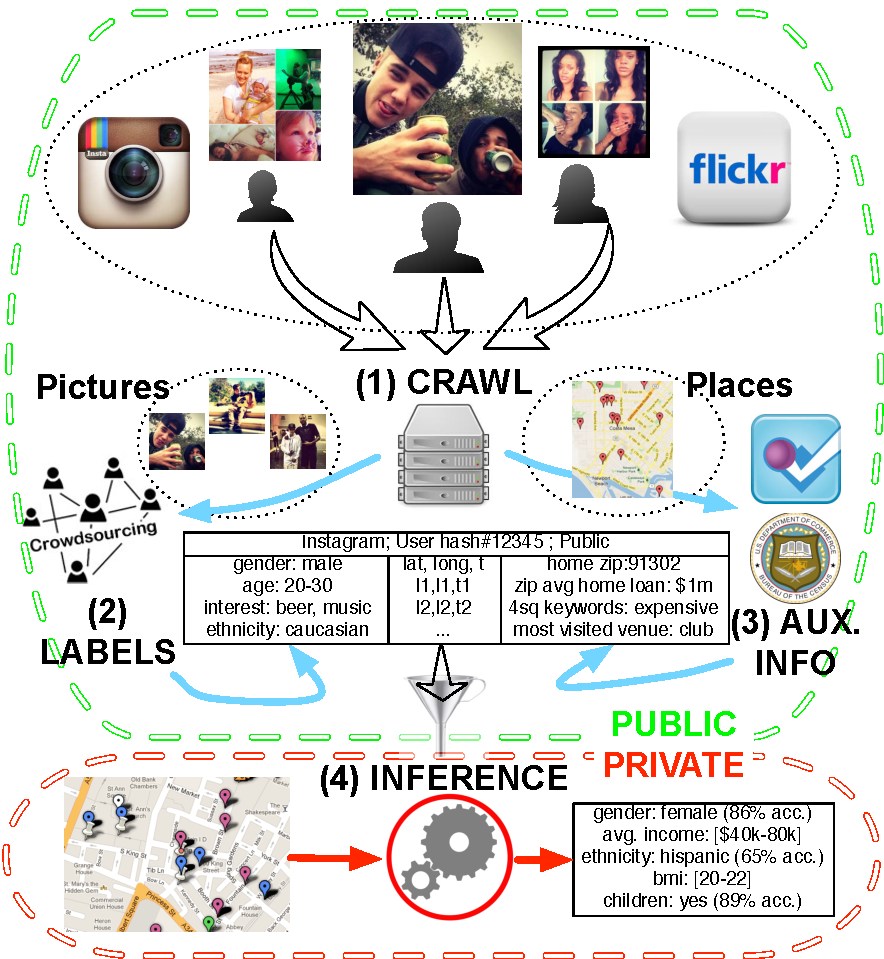
\includegraphics[width=\linewidth]{fig/footprints/system.pdf}
	\end{center}
	\caption{Methodology overview. 
	% A mobility dataset can be built in the following steps: (1) Public user profiles of a photosharing service are crawled and photo metadata are extracted into a database (Data Collection). (2) Corresponding photos are labeled (with labels for ethnicity, gender, etc.) by crowd workers in an online labor marketplace (User Labeling). (3) The dataset is further enhanced with auxiliary data, e.g., with the information that a certain location is close to a restaurant (Adding Auxiliary Information). (4) The dataset can then be used to analyze attributes on various demographic levels or train and test classifiers for individual inferences.
	}
	\label{fig:system}
\end{wrapfigure}
% \end{figure}

% \paragraph{Data Collection} 
\textbf{Data Collection.} 
We collected publicly available photo metadata from Instagram covering data for the years from 2011 through 2013. 
This data collection and use was exempt from user informed consent under our institution's IRB rules since (1) we only collected publicly available online metadata, (2) after we used the metadata and the users were labeled, any identifying information, such as usernames, were removed, and (3) we only kept track of users' identities separately and for one single purpose (ensuring that the data we collected still belongs to a public Instagram  profile). 
We started our crawl from a root user (the founder of Instagram, on whose feed a large and diverse group of users comment) and followed further users subsequently through comments and likes. 
We skipped users with no geotagged photo in their first 45 photos. 
Our crawl retrieved a total of 35,307,441 photo location points belonging to 118,374 unique users.

% \paragraph{User Labeling} 
\textbf{User Labeling}.
We labeled users for gender and ethnicty, first doing a manual comparison of trusted labelers before scaling with crowdsourcing.
We selected a subset of profiles to label, being unable to label the entire dataset due to cost.
In order to compare our data set to previous studies~\cite{Isaacman:2011un,Isaacman:2011cn,Isaacman:2010en}, we selected users from the Los Angeles (LA) and New York City (NY) metropolitan areas, based on a majority of a user's locations being in this area to filter out tourists.
% To match previous studies~\cite{Isaacman:2011un,Isaacman:2011cn,Isaacman:2010en} that leveraged ZIP codes of CDR billing addresses from the Los Angeles (LA) and New York City (NY) metropolitan areas we randomly chose users from those areas as well. 
% A user's home is the ZIP code where he or she had the most checkins (that is, photos taken). Note that this mitigates the content produced by tourists and other occasional visitors to LA and NY unless those have no other Instagram activity. 
% A combination of workers on Amazon Mechanical Turk (MTurk) and undergraduate students were asked to annotate users' ethnicities and gender based on the users' photos. 
% However, in order to ensure that user pictures on Instagram profiles are sufficient to make a conclusive determination of users' ethnicities and genders we ran a preliminary experiment by selecting 200 profiles at random (excluding celebrities and business accounts) and having each labeled independently by two undergraduate students. 
We ran a preliminary experiment by selecting 200 profiles at random (excluding celebrities and business accounts) and labeleing each independently by two undergraduate students.
We observed a strong agreement on gender (98\%).
For ethnicity labeling we leveraged United States Census categories, asking the student annotators to categorize each user either as Hispanic or Latino (Hispanic), White alone (Caucasian), Black or African American alone (African American), or Other (combining all remaining Census categories, including Asian).
% Merging all remaining Census fields in the last category limits our detail view, although we would otherwise have some annotations being quite rare. 
Just as in the Census, our Hispanic category includes Hispanics and Latinos of any race, while the remaining categories do not include any Hispanics or Latinos. 
We found that our profiles are diverse: 45\% Caucasian, 21\% Hispanic, 15\% African American, and 19\% Other.
The students' labels matched 87\% of the time and when evaluated as a binary classification task (Caucasian vs. all other categories) the agreement reached 94\%. 
We note that the two labeling students were of different gender and ethnicity themselves. 
% In conclusion, despite sparse data and ethnicity spanning a continuous spectrum, we found that labels are surprisingly predictable and consistent across annotators. 
% As studies confirmed that 91\% of teens post a photo of themselves on social networks~\cite{PewTeen} and that 46.6\% of photos are either selfies or show the user posing with other friends~\cite{ICWSM148118} there is also evidence in many cases that it is actually the account owner who is shown in the pictures.

% \begin{figure}[htp]
\begin{wrapfigure}{R}{0.5\textwidth}
	\centering
	\begin{subfigure}[t]{1.22in}
		\centering
		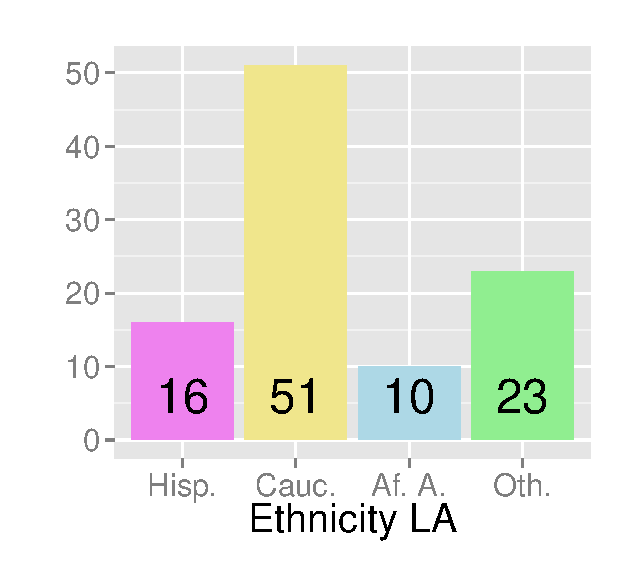
\includegraphics[width=1.22in]{fig/footprints/la_eth_bar.eps}
	\end{subfigure}
	\begin{subfigure}[t]{1.22in}
		\centering
		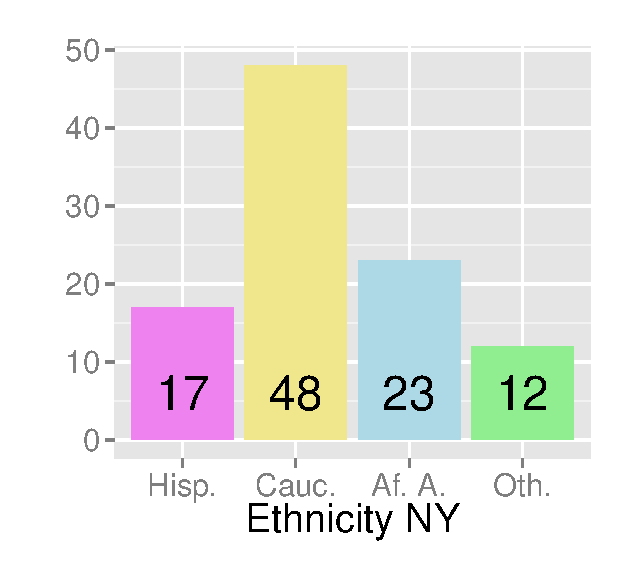
\includegraphics[width=1.22in]{fig/footprints/ny_eth_bar.eps}
	\end{subfigure}
	\begin{subfigure}[t]{0.7in}
		\centering
		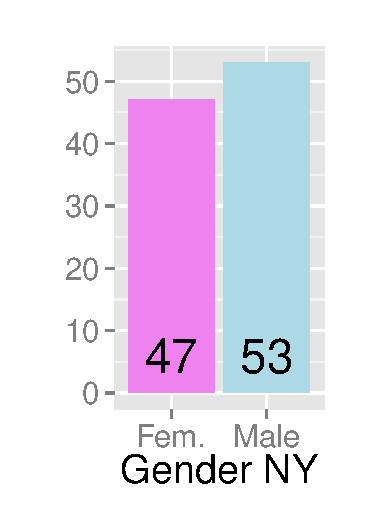
\includegraphics[width=0.7in]{fig/footprints/ny_gender_bar.eps}
	\end{subfigure}
{\small
\begin{tabular}{| l | c | c | c |}
\hline
                          & {\textit{Ethnicity LA}} & {\textit{Ethnicity NY}} & {\textit{Gender NY}} \\ \hline
{\textit{Users (n)}}      & 427                     & 588                     & 241 \\ \hline
K.'s $\alpha$ Multi.      & \textbf{0.74}           & \textbf{0.68}           & -   \\ \hline
K.'s $\alpha$ Binary      & \textbf{0.78}           & \textbf{0.74}           & \textbf{0.85} \\ \hline
\end{tabular}
}
\vspace{0.7ex}
	\caption{Annotations for LA and NY. Top: percentages of user labels for the different categories. Bottom: absolute numbers of labeled users and annotation agreement results.}
	\label{fig:demographics}
% \end{figure}
\end{wrapfigure}


We scaled our annotation using Amazon Mechanical Turk workers, with each profile labeled by two MTurk workers.
In cases of disagreement between the MTurk annotators we asked one of our undergraduate annotators for an additional label to break the tie or assign a label from a different third category. We decided to use a tiered annotation mechanism with the undergraduate annotator making the final decision in case of disagreements.
We ran this on two different days, with workers paid \$0.10 per profile on the first day and \$0.05 on the second.
This resulted in 1,015 labeled profiles.
The undergraduate annotator was compensated the regular stipend at our institution.
% To scale our annotation, we asked MTurk annotators to label a larger number of profiles for the same metropolitan areas using the same label categories. For consistency, we did not reuse the profiles used for the preliminary experiment described above. Each profile was labeled by two MTurk annotators. In cases of disagreement between the MTurk annotators we asked one of our undergraduate annotators for an additional label to break the tie or assign a label from a different third category. We decided to use a tiered annotation mechanism with the undergraduate annotator making the final decision in case of disagreements as unsupervised crowd workers on MTurk or similar platforms tend to be less attentive than physically available workers~\cite{Paolacci10runningexperiments}, who also have the possibility to ask clarifying questions. We were also careful to not drop any labels to avoid the introduction of a systematic annotation bias. Over two days 117 MTurk annotators participated in our task resulting in 1,015 properly labeled users with the labels shown in Figure~\ref{fig:demographics}. On the first day the annotators were compensated \$0.10 per annotation and on the second day \$0.05. The undergraduate annotator was compensated the regular stipend at our institution.
In order to measure the quality of agreement among the annotators we made use of Krippendorff's $\alpha$~\cite{Krippendorff}, as shown in Figure~\ref{fig:demographics}.
% Generally, values above 0.8 are considered as good agreement, values between 0.67 and 0.8 as fair agreement, and values below 0.67 as dubious~\cite{Manning:2008:IIR:1394399}. Figure~\ref{fig:demographics} shows that we obtained fair and good agreement and, thus, reliable ground truth for both our ethnicity and gender classifications. 
We collected auxiliary information mapping locations to the race and gender of residents using the United States Census~\cite{census:2010} and location to categories using Foursquare's reverse-geocoding API.

% \paragraph{Adding Auxiliary Information}
% %\textbf{Adding Auxiliary Information}.
% We collected auxiliary information from two sources. First, for the comparative analysis of demographic patterns with our data in \S\ref{sec:demographic-patterns} we used data from the Census~\cite{census:2010} to associate geographic regions with gender and ethnicity distributions. 
% Throughout the study we use Census-defined geographic granularities, ranging from block groups of 600-3k people to neighborhood tabulation areas (NTAs; 15k people), public use microdata areas (PUMAs; 100k people), and counties with populations of up to 2.6 million.
% We adjusted the distributions by ethnicity- and gender-specific Internet \cite{file:2013,PewSocialMedia2012} and Instagram \cite{Pew2012} usage numbers. As explained in~\S\ref{sec:demographic-patterns} we also took into account that Caucasian Hispanics are often perceived as Caucasian alone~\cite{MelaninMillennium}. Second, for each checkin we obtained Foursquare information on the ten closest venues. We then used Foursquare's average venue popularities and venue categories as features for our inference algorithms (\S\ref{sec:inference}) since those features could provide an estimate of the types of places a user would visit.

% \section{Mobility-Demographics}
% \label{sec:patterns}
% We now present a mobility pattern analysis for various population levels. Our dataset reveals mobility trends similar to those of CDRs (\S\ref{sec:mobility-patterns}) and generally represents the adjusted Census population well (\S\ref{sec:demographic-patterns}). In many cases we are able to detect differences in mobility patterns between ethnic groups and genders that can be plausibly explained by previous sociological findings (\S\ref{sec:mobility-patterns-by-Demographic}), and we are also able to detect segregation among ethnic groups (\S\ref{sec:ethnic-segregation}).

\subsection{Mobility Patterns}
\label{sec:mobility-patterns}

In order to compare the mobility patterns of our dataset to those in the CDR dataset of~\cite{Isaacman:2011cn,Isaacman:2010en} we only consider checkins for the years 2011 through 2013 each for the Spring months from March 15 to May 15 and for the Winter months from November 15 to January 31 (the LA and NY Spring and Winter subsets, respectively). Table \ref{tab:basics} shows the distribution of the data in our subsets compared to those in the CDR dataset~\cite{Isaacman:2011cn}. The mobility traces from our subsets are much more sparse. Most notably, while the CDR dataset has at least eight location points from call activity per day for the median user in LA and NY---and even 12 if text messages are added---the data in all of our subsets account for only one location point for the median user per day.

\begin{table}[t]
\centering
{\small
\begin{tabular}{| l | c | c | c | c | c | c | c |}
\hline
 & \multicolumn{2}{c|}{\textit{Spring}}& \multicolumn{2}{c|}{\textit{Winter}}  \\ \hline
\textit{Statistic} & LA          & NY           & LA          & NY \\ \hline
Total Checkins     & 135,503     & 109,506      & 118,446     & 98,286  \\
(Total CDRs)       & (74M)       & (62M)        & (247M)      & (161M) \\ \hline
Min. Loc./Day      & 1           & 1            & 1           & 1 \\ \hline
1st Qu. Loc./Day   & 1           & 1            & 1           & 1 \\ \hline
Med. Loc./Day      & \textbf{1}  & \textbf{1}   & \textbf{1}  & \textbf{1} \\
(Med. Calls/Day)   & \textbf{(9)}& \textbf{(10)}& \textbf{(8)}& \textbf{(9)} \\ 
(Med. Texts/Day)   & -           &  -           & \textbf{(4)}& \textbf{(3)} \\ \hline
Mean Loc./Day      & 1.97        & 2.12         & 1.96        & 2.1 \\ \hline
3rd Qu. Loc./Day   & 2           & 2            & 2           & 2 \\ \hline
Max Loc./Day       & 73          & 62           & 98          & 69 \\ \hline		
\end{tabular}
}
\caption{Statistics of our LA and NY subsets compared to the CDR dataset in~\protect\cite{Isaacman:2011cn} (where available, in parentheses). Our calculations do not consider any day where a user had no checkins.}
\label{tab:basics}
\end{table}

Another insightful metric for comparing mobility patterns is the \emph{daily range}, defined as the maximum straight line distance a phone has traveled in a single day~\cite{Isaacman:2010en}. Daily ranges are characteristic for mobility because, for example, median daily ranges on weekdays represent a lower bound for a commute between home and work locations~\cite{Isaacman:2010en}. Figure~\ref{fig:ranges} shows a subset of our results. Our ranges are generally smaller than those reported by~\cite{Isaacman:2011cn,Isaacman:2010en}. However, the general trends in both datasets are similar. Most importantly, people in LA have generally greater ranges than people in NY. Also, in both areas people tend to travel longer during the day than at night. However, there are also differences: according to our data New Yorkers in the 98th percentiles travel farther than Angelinos.

\begin{figure}[t]
	\centering
	\begin{subfigure}[t]{1in}
		\centering
		\includegraphics[width=1in]{fig/footprints/max_ranges.eps}
    % \includegraphics[width=1in]{fig/max_ranges.eps}
	\end{subfigure}
	\begin{subfigure}[t]{1in}
		\centering
    \includegraphics[width=1in]{fig/footprints/med_ranges_day.eps}
		% \includegraphics[width=1in]{fig/med_ranges_day.eps}
	\end{subfigure}
	\begin{subfigure}[t]{1in}
		\centering
    \includegraphics[width=1in]{fig/footprints/med_ranges_night.eps}
		% \includegraphics[width=1in]{fig/med_ranges_night.eps}
	\end{subfigure}
	\vspace{2ex}

	{\small
\begin{tabular}{| l | c | c | c | c | c | c | c | c | c |}
\hline
           & \multicolumn{2}{c|}{\textit{Max. Mo.--Fr.}} & \multicolumn{2}{c|}{\textit{Med. Mo.--Fr.}} & \multicolumn{2}{c|}{\textit{Med. Night}}  \\ \hline
\%       & LA       & NY       & LA      & NY      & LA      & NY \\ \hline
98       & 2,471.7  & 3,625.6  & 133     & 209.9   & 117.4   & 129.9 \\
         & (2,467)  & (2,455)  & (32)    & (29)    & (23.1)  & (19.4) \\ \hline
75       & 47.5     & 37       & 9.3     & 5.3     & 6.1     & 3.3 \\
         & (130)    & (111)    & (10)    & (8.2)   & (8)     & (5.6) \\ \hline
50       & \textbf{12.8}     & \textbf{8.1}        & \textbf{4}   & \textbf{2.2}   & \textbf{1.6}   & \textbf{1} \\
         & (36)     & (27)     & (5)     & (3.8)   & (4)     & (2.6) \\ \hline
25       & 3        & 2.3      & 0.8     & 0.5     & 0.1     & 0.1 \\
         & (17)     & (12)     & (2)     & (1.3)   & (1.4)   & (0.7)\\ \hline
02       & $\epsilon$ & $\epsilon$ & $\epsilon$& $\epsilon$& $\epsilon$& $\epsilon$ \\
         & (1.6)    & (1.3)    & (0)   & (0)   & (0)   & (0)\\ \hline
\end{tabular}
}
	\caption{Daily ranges in miles. Top: boxes show the 25th, 50th, and 75th percentiles; whiskers the 2nd and 98th percentiles. Bottom: table with the percentiles represented in the boxplots. The maximum range (Max. Mo.--Fr.) is a user's longest distance and the median range (Med. Mo.--Fr.) a user's median distance, each taken on a single day for the entire Spring subset on a weekday~\protect\cite{Isaacman:2010en}. The median range at night (Med. Night) represents the median distance a user has traveled on a day for the entire combined Spring and Fall subset from 7pm--7am ~\protect\cite{Isaacman:2011cn}. Previous results~\protect\cite{Isaacman:2011cn,Isaacman:2010en} are shown in parentheses. Our calculations do not consider any day where a user had a zero range, that is, had multiple checkins at the same location or a single checkin only. We define $\epsilon<0.005$ miles.}
\label{fig:ranges}
\end{figure}

\subsection{Demographic Patterns}
\label{sec:demographic-patterns}

As our LA and NY subsets are annotated with ethnicity and gender labels (\S\ref{sec:method}) we are able to compare the resulting demographic distributions to the respective Census distributions. However, initial comparisons reveal substantial differences. For example, according to the Census there are more females than males (53\% vs. 47\%) living in Kings County~\cite{census:2010} while our observed label frequencies suggest that there should be substantially fewer (43\% vs. 57\%). This result is even more surprising as the gender-specific usage rates of Internet (70\% vs. 69\%)~\cite{file:2013} and Instagram (16\% vs. 10\%)~\cite{Pew2012} should further increase the percentage of females beyond the Census. However, while 86\% of female social network account owners set their profile to private, only 74\% of males do so~\cite{PewSocialMedia2012}. Adjusting the Census distribution for this difference (as well as for gender-specific Internet and Instagram usage rates) leads to a distribution of females and males (49\% vs. 51\%) much closer to the distribution we observed for our labels.

Similarly to gender, we make adjustments to the Census distributions for the varying percentages of Internet and Instagram usage rates among different ethnicities as well. However, even then we still observed a substantial Hispanic underrepresentation, which was also observed for the southwest of the United States by~\cite{mislove-2011-twitter}. We found this phenomenon difficult to assess, specifically, as ethnicity is not significant for setting a profile private~\cite{journals/jcmc/LewisKC08}, activity levels (posting pictures, etc.) are not lower for Hispanics~\cite{statista}, and our annotation disagreements are not higher when the Hispanic label is involved. However, we believe that the reason for the underrepresentation is the perception of Caucasian Hispanics as Caucasian alone. In a study, six of seven Caucasian Hispanics reported that others see them as Caucasian alone~\cite{MelaninMillennium}. Therefore, we believe that most Caucasian Hispanics were actually labeled as Caucasian (i.e., our annotators agreed on an incorrect classification). Thus, we adjusted the observed label frequencies by adding to the Hispanic labels a number of labels corresponding to the Census percentage of Caucasian Hispanics and subtracting the same number from the Caucasian labels.

\begin{figure}[t]
  \centering
  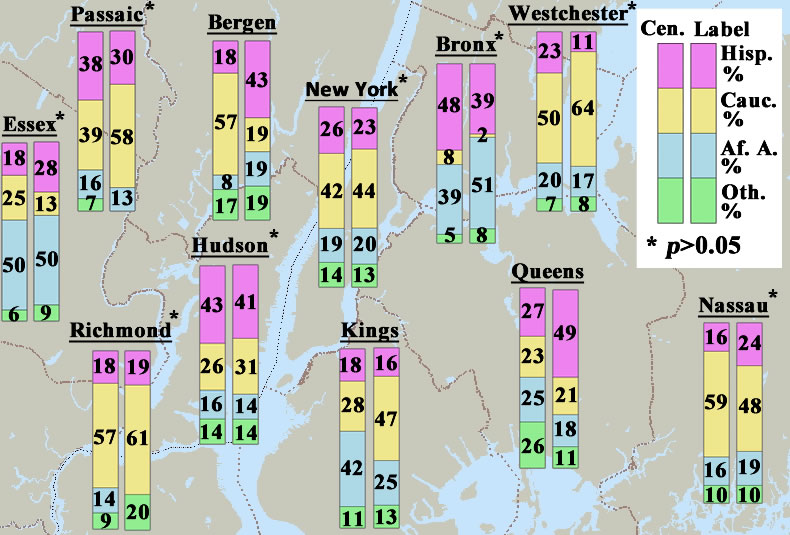
\includegraphics[width=3.35in]{fig/footprints/map.jpg}
	\vspace{0.2ex}

{\small
\begin{tabular}{| l | c | c | c | c | c |}
\hline
 & \multicolumn{2}{c|}{\textit{Ethnicity Multi-Cat.}} & \multicolumn{2}{c|}{\textit{Ethnicity Binary}} & \textit{Gender}  \\ \hline
\textit{Gran.} & LA       & NY                & LA      & NY                              & NY \\ \hline
State          & 0/1      & 0/1               & 1/1     & 0/1                             & 1/1 \\
               & (0\%)    & (0\%)             & (100\%) & (0\%)                           & (100\%) \\ \hline
County         & 1/2      & \textbf{8/11}     & 2/2     & 6/8                             & 4/4 \\
               & (50\%)   & \textbf{(73\%)}   & (100\%) & (75\%)                          & (100\%) \\ \hline 
PUMA           & 12/16    & 11/17             & 2/2     & 5/6                             & 1/1\\ 
               & (75\%)   & (65\%)            & (100\%) & (83\%)                          & (100\%) \\ \hline
NTA            & -        & 9/16             & -       & 7/7                             & 2/2\\
               & -        & (56\%)            & -       & (100\%)                         & (100\%) \\ \hline
ZIP            & 3/3      & 8/14              & 1/1     & 3/3                             & -  \\
               & (100\%)  & (57\%)            & (100\%) & (100\%)                         & - \\ \hline
\end{tabular}
}
\caption{Chi square goodness of fit test results for ethnicity and gender at various levels of Census-defined granularity. Top: detailed view of the multi-category ethnicity distributions for the NY county level. Left bars show the Census distributions (Cen.) and right bars the label distributions (Label). Bottom: complete results of the chi square tests. NTAs are specific to NY and not available for LA. Below the ZIP code and NTA levels we did not have enough data to perform chi square tests. We follow ~\protect\cite{Roscoe:1971} and require the average expected frequency for a chi square test with more than one degree of freedom to be at least two and for a test with one degree of freedom to be at least 7.5. To prevent skewing due to small sample sizes we also use a Monte Carlo simulation with 2,000 replicates.}
\label{fig:map}
\end{figure}

\begin{figure}[t]
	\centering
    \includegraphics[width=3.35in]{fig/footprints/max_ranges_eth_ny.eps}
		% \includegraphics[width=3.35in]{fig/max_ranges_eth_ny.eps}
    \includegraphics[width=3.35in]{fig/footprints/med_ranges_gender_ny.eps}
		% \includegraphics[width=3.35in]{fig/med_ranges_gender_ny.eps}
	\vspace{0.1ex}

{\small
\resizebox{\columnwidth}{!}{%
\begin{tabular} {| l | c | c | c | c | c | c |}
\hline
           & \multicolumn{4}{c|}{\textit{Max. Mo.-Fr. NY}} & \multicolumn{2}{c|}{\textit{Med. Night NY}}  \\ \hline
\%           & Hisp.   & Cauc.   & Af. A.  & Oth.    & Fem.  & Male \\ \hline
98           & 2,480.8 & 6,509.4 & 2,270.9 & 6,788.1 & 9.8   & 11.5 \\ \hline
75           & 50.8    & 592.3   & 44      & 187     & 3.2   & 4.7 \\ \hline 
50           & \textbf{13.5}    & \textbf{52.1}    & \textbf{11.9}    & \textbf{18.4}    & \textbf{1.8}   & \textbf{1.9} \\ \hline 
25           & 4.9     & 7       & 5.5     & 3.7     & 0.4   & 0.6 \\ \hline 
02           &$\epsilon$&$\epsilon$&$\epsilon$&$\epsilon$&$\epsilon$&$\epsilon$\\ \hline 
\end{tabular}
}}
	\caption{Daily ranges in miles. Top: density plot of the maximum daily ranges by ethnicity. Middle: density plot of the median daily ranges at night by gender. Bottom: table with the percentiles of the daily ranges represented in the plots. We rounded extremely small daily ranges up to 0.005 miles. Our calculations do not consider any day where a user had a zero range, that is, had multiple checkins at the same location or a single checkin only. We define $\epsilon<0.005$ miles.}
	\label{fig:ranges_ny}
\end{figure}

We perform chi square tests for goodness of fit comparing the gender and ethnicity distributions of our labels to the corresponding Census distributions for different levels of granularity. In most cases we obtain a value of $p>0.05$ and find no evidence to reject the null hypothesis that the observed gender and ethnicity distributions follow the corresponding Census distributions. For example, as shown in Figure~\ref{fig:map}, for eight out of 11 counties in the NY area our tests resulted in $p>0.05$ providing no evidence that our multi-category ethnicity distributions deviate significantly from the Census distributions. However, there are also cases with differences. It is no surprise that this is true for the state level as our distributions only cover users from the LA and NY metropolitan areas. However, overall we believe our results suggest that geotag data often replicate demographic trends faithfully.

\subsection{Mobility Patterns by Demographic}
\label{sec:mobility-patterns-by-Demographic}

By combining our methodologies from the previous two subsections we now show the differences in mobility patterns between ethnic groups and between males and females, respectively. In particular, we examine differences in daily ranges, home ranges, and temporal checkin characteristics.

\paragraph{Daily Ranges}

Figure~\ref{fig:ranges_ny} shows some of our daily range results for ethnic groups and genders based on our sets of labeled users for LA and NY. We obtained the same types of daily ranges as described earlier in Figure~\ref{fig:ranges}, however, this time for all days of the year. It is striking that Caucasians generally have a higher maximum daily range than the other ethnic groups. Indeed, a two sample Kolmogorov-Smirnov test reveals that the Caucasian range distribution differs significantly ($p<0.05$) from the African American and Hispanic distribution. This result illustrates a more general finding: daily ranges of Caucasians often differ significantly from those of minorities. For 44\% (8/18) of the comparisons of a Caucasian distribution to a minority distribution (three comparisons for maximum weekday, three for median weekday, three for median at night---each for LA and NY) the difference is significant at the 0.05 level. However, for the comparisons among minority distributions we only find 6\% (1/18) to be significantly different from each other. 

The differences in ranges by ethnicity can be most prominently observed in the comparisons of Caucasians to African Americans and to Hispanics. However, it should be noted that at night all ethnicities exhibit very similar ranges. This finding stands in contrast to the difference in daily ranges between males and females. In fact, the only statistically significant difference ($p<0.05$) that we observed between male and female ranges occurs for the median daily ranges at night. As shown in Figure~\ref{fig:ranges_ny}, females tend to travel smaller distances at night than males. There are many possible explanations for this phenomenon. One reason could be that women travel fewer times at night due to safety concerns~\cite{badger:2014} and, consequently, also avoid longer trips. In general, for both males and females---as well as for all ethnicities---we find that our observed daily ranges follow a (skewed) log normal distribution.

\paragraph{Home Ranges}

In order to evaluate differences in mobility with respect to an individual's home location we complement the analysis of daily ranges with the evaluation of \emph{home ranges}. A home range is a straight line distance between someone's home and another place to which the person travels. Different from daily ranges we calculate the home ranges not on a daily basis, but instead consider all home ranges---whether they were the maximum travel distance for a day or not. Based on a user's home location, as specified in \S\ref{sec:method}, we calculate the distance between the home and each checkin for the different ethnic groups and genders. Figure~\ref{fig:checkin_distance} shows the resulting CCDFs for the home ranges of the NY users.

\begin{figure}[h]
  \centering
  \includegraphics[width=\linewidth]{fig/footprints/distance_ccdf_eth_wide.eps}
  % \includegraphics[width=\linewidth]{fig/distance_ccdf_eth_wide.eps}
  \includegraphics[width=\linewidth]{fig/footprints/distance_ccdf_gender_wide.eps}
  % \includegraphics[width=\linewidth]{fig/distance_ccdf_gender_wide.eps}
  \caption{CCDFs of home ranges for NY. Top: CCDFs for different ethnic groups. Bottom: CCDFs for males and females.}
  \label{fig:checkin_distance}
\end{figure}

Both graphs show a noticeable decrease around the 2,500 mile mark, which is the distance from NY to major hubs on the West Coast of the United States (most notably LA (2,475 miles), San Francisco (2,563 mi), and Seattle (2,405 miles)). Males and females have very similar home ranges at the edges of the graph. However, females travel farther in the medium home ranges. This finding could be based on the fact that women generally take more often vacations~\cite{kelton:2013} and travel longer distances to work when they are employed full-time~\cite{kwan:1999}. It should be noted that the larger home ranges are not inconsistent with the previous observation of shorter ranges for females at night as that result does obviously not consider ranges during the day. The plot for ethnicity is in line with our previous observation that Caucasians travel farther from home than minorities.

\paragraph{Temporal Checkin Characteristics}

\begin{figure}[t]
  \centering
  \includegraphics[width=0.49\linewidth]{fig/footprints/time_hist_all_norm.eps}
  % \includegraphics[width=0.49\linewidth]{fig/time_hist_all_norm.eps}
  \includegraphics[width=0.49\linewidth]{fig/footprints/time_hist_eth_norm.eps}
  % \includegraphics[width=0.49\linewidth]{fig/time_hist_eth_norm.eps}
  \caption{Histograms of checkin times for NY. Left: Comparison of weekends and weekdays for all user groups. Right: Comparison of Caucasian and minority user groups for weekends and weekdays. Dashed lines correspond to weekends, solid lines to weekdays.}
  \label{fig:time_activity}
\end{figure}

Beyond spatial differences we explore differences in temporal activity as well. Figure~\ref{fig:time_activity} shows histograms for checkins by hour of day. As might be expected, we observe periodic behaviors with low checkin levels between 4--6am and peak levels from 3--8pm. On weekends the lows occur at later times than on weekdays suggesting that users wake up later on weekends. We also see a dramatic increase in activity after 5pm on weekdays, which could correspond to the time at which many users get off of work. When broken up into Caucasians and minorities, we see fairly similar curves, except with a more pronounced weekday after-work increase for minorities. It could be the case that Caucasians work more often in flexible environments. We observe no substantial differences between genders or NY and LA.

\subsection{Ethnic Segregation}
\label{sec:ethnic-segregation}

Location data are the basis for measuring residential segregation, that is, the degree to which two or more groups live separately from one another in different parts of the urban environment~\cite{masseyAndDenton}. Trends in residential segregation characterize a group's proximity to community resources (e.g., health clinics) and its exposure to environmental and social hazards (e.g., poor water quality and crimes)~\cite{Reardon}. In addition to \emph{residential} segregation we also introduce and evaluate \emph{mobility} segregation, which we understand as the degree to which two or more groups \emph{move} to and from different parts of an area. Mobility segregation allows for a dynamic view of segregation, for example, in order to determine a group's ease of access to community resources away from home.
\\
\\

\paragraph{Methodology}
Various intersecting dimensions of segregation can be distinguished~\cite{masseyAndDenton}. We explore two standard measures, each for a different dimension: the interaction index measures the dimension of exposure (the extent to which minority group members are exposed to majority group members in an area~\cite{masseyAndDenton}) and the entropy index measures the dimension of evenness (the extent to which minority group members are over- or underrepresented in an area~\cite{masseyAndDenton}). The interaction index, $B$, can be understood as the probability of a minority group member interacting with a majority group member and is defined~\cite{White} by

\begin{equation}
\label{interaction}
	B_{kl} = \sum (\frac{n_{ik}}{N_k})(\frac{n_{il}}{n_i}),
\end{equation}

\noindent where $n_{ik}$ is the population of ethnic minority group $k$ in area $i$ (e.g., in a ZIP code area), $N_k$ is the number of persons in group $k$ in the total population of all areas, $n_{il}$ is the population of ethnic majority group $l$ in area $i$, and $n_i$ is the area population.

The entropy index was used in social network research before \cite{Cranshaw:2010:BGP:1864349.1864380} and has the advantage over other indices that it can be used to measure segregation for more than two groups. We define the entropy index~\cite{White}, $H$, as

\begin{equation}
\label{entropy1}
	H = \frac{H^* - \bar{H}}{H^*},
\end{equation}

\noindent where $H^*$ is the population-wide entropy defined by

\begin{equation}
\label{entropy2}
	H^* = - \sum\limits_{k=1}^K P_k ln (P_k),
\end{equation}

\noindent and $\bar{H}$ is the weighted average of the individual areas' entropies defined by 

\begin{equation}
\label{entropy3}
	\bar{H} = - \sum\limits_{i=1}^I \frac{n_i}{N} \sum\limits_{k=1}^K P_{ik} ln (P_{ik}),
\end{equation}

\noindent where $K$ is the number of different ethnic groups, $P_k$ is the proportion of ethnicity $k$ in the total population, $I$ is the number of different areas, $n_i$ is the population in an area, $N$ is the sum of the population from all areas, and $P_{ik}$ is the proportion of the population of ethnicity $k$ in area $i$ (while it is defined that $P_{ik} ln (P_{ik}) = 0$ for $P_{ik} = 0$).

For both interaction and entropy indices we make use of our sets of labeled users for LA and NY, however, exclude all areas for which the label distribution deviated significantly from the Census distribution as indicated by $p\leq0.05$. Thus, for example, as shown in Figure~\ref{fig:map}, on the county level we do not include Queens, Kings, and Bergen. These exclusions are necessary as otherwise the accuracy of our results decreases substantially. Recall that we define a user's home as the ZIP code where he or she had the most checkins (\S\ref{sec:method}) and that we adjust label and Census distributions (\S\ref{sec:demographic-patterns}).

\paragraph{Residential Segregation}

\begin{table}[t]
\centering
{\small
\begin{tabular}{| l | c | c | c | c | c | c |}
\hline
 & \multicolumn{2}{c|}{\textit{Hisp./Cauc.}} & \multicolumn{2}{c|}{\textit{Af. A./Cauc.}} & \multicolumn{2}{c|}{\textit{Oth./Cauc.}} \\ \hline
\textit{Gran.} & LA       & NY       & LA       & NY       & LA       & NY       \\ \hline
County         & 0.29     & 0.34     & 0.27     & 0.3     & 0.3        &  0.4    \\
               & (-2\%)   & (+2\%)   & (+1\%)   & (-2\%)   & (-3\%)    & (0\%) \\ \hline 
PUMA           & 0.32     & \textbf{0.39}     & 0.43     & 0.42     & 0.31     &  0.49    \\
               & (-6\%)   & \textbf{(+3\%)}   & (+4\%)    & (+7\%)   & (-10\%)  & (+5\%) \\ \hline 
NTA            & -        & 0.54     & -        & 0.43     & -        & 0.55     \\
               & -        & (+6\%)   & -        & (+3\%)  & -        & (+7\%) \\ \hline 
ZIP            & 0.36     & 0.56     & 0.33     & 0.55     & 0.58     &  0.5    \\
               & (-19\%)  & (0\%)   & (-23\%)   & (+1\%)   & (-1\%)   & (-7\%) \\ \hline
$\varnothing$ \% Diff.       & \multicolumn{2}{c|}{\textbf{5\%}} & \multicolumn{2}{c|}{\textbf{6\%}} & \multicolumn{2}{c|}{\textbf{5\%}} \\ \hline
\end{tabular}}
\caption{Interaction index ($B$) for different granularities based on labeled Instagram data. Differences to the interaction index calculated from Census data are shown in percentage points in parenthesis. For example, the probability of a Hispanic person to interact with a Caucasian person on the PUMA granularity level for NY is 39\%. However, as shown in parenthesis, this result is an overestimation by three percentage points over the Census distribution probability of 36\%. The last row of the table shows the mean difference between our labels and the Census for the three different ethnicities in absolute percentage points for both LA and NY together. Note that NTAs are not available for LA and that we also did not analyze the state level as the label and Census distributions differ significantly (Figure \ref{fig:map}).}
\vspace{2mm}
\label{tab:interaction}
\end{table}



\begin{table}[t]
\centering
{\small
\begin{tabular}{| l | c | c | c | c | c |}
\hline
 & \multicolumn{5}{c|}{\textit{Entropy}} \\ \hline
\textit{Metro} & County   & PUMA    & NTA    & ZIP    & $\varnothing$ \% Diff.  \\ \hline
LA             & 0.01     & 0.15    & -      & 0.15   & \multirow{4}{*}{\textbf{3\%}}  \\
               & (-2\%)   & (+8\%)  & -      & (+9\%) &  \\ \cline{1-5} 
NY             & 0.08     & 0.14    & 0.08   & 0.09   &  \\
               & (0\%)    & (+1\%)  & (0\%)  & (+4\%) &  \\ \hline
\end{tabular}
}
\caption{Entropy index ($H$) for different granularities based on labeled Instagram data. Differences to the entropy index calculated from Census data are shown in percentage points in parenthesis. As explained in Table \ref{tab:interaction}, the last column shows the measurement error. As further explained in Table \ref{tab:interaction}, we did not consider NTA (LA) and state granularities (LA and NY).}
\label{tab:entropy}
\end{table}

Tables~\ref{tab:interaction} and~\ref{tab:entropy} show our results for the interaction and entropy indices, respectively. For the most part the interaction between Caucasian and minority group members can be considered fairly high~\cite{IcelandDemographic}. All three minorities in LA and NY have similar probabilities of interacting with Caucasians. The measurement errors of 5\% (Hisp./Cauc. and Oth./Cauc.) and 6\% (Af. A./Cauc.) between our labeled data and the Census suggest that our results are overall reliable. The inaccurate results for LA on the ZIP code level appear to have been caused by the smaller number of data points. While the level of interaction seems to increase when areas become more fine-grained, this phenomenon seems to be caused by the different area coverage for the various granularities. For example, it is not present when considering all NY city areas, where the Census distributions for the interaction of African Americans and Caucasians are: 0.41 (County), 0.25 (PUMA), 0.2 (NTA), and 0.22 (ZIP).

With entropy index scores ranging from 0.01 to 0.15, as shown in Table~\ref{tab:entropy}, we find another indicator for low segregation~\cite{IcelandDemographic}. However, it should be noted that this low level of segregation is a characteristic of the particular areas we investigated. For example, for all NY city areas at the NTA level we calculated an entropy of 0.31 indicating higher segregation. However, with mean differences of 5\% (Hisp./Cauc.) and 6\% (Af. A./Cauc. and Hisp./Oth.) between the results for our labeled data and the Census-based calculation our findings are generally reliable. As in the case of interaction, we believe that any existing inaccuracies could be due to small numbers of data points.

\paragraph{Mobility Segregation}

We evaluate mobility segregation based on the same measures as residential segregation---interaction and entropy indices. However, instead of using home locations we leverage checkin data. More specifically, for each user we calculate the percentage that he or she spent at a certain area and sum the resulting values for all users of a certain ethnicity. This method aims to avoid overcounting of active users. Our results are shown in Table~\ref{tab:interactionEntropy} and indicate that segregation levels in terms of where people go are similar to levels of where people live. Indeed, it would have been surprising to see higher segregation levels as members of minority groups may work in predominantly Caucasian areas. Furthermore, it would also have been a surprise to see lower levels of segregation as residential segregation is already relatively low.

\begin{table}[h]
\centering
{\small
\begin{tabular}{| l | c | c | c | c |}
\hline
 & \multicolumn{3}{c|}{\textit{Interaction}} & \textit{Entropy} \\ \hline
\textit{Metro} & Hisp./Cauc. & Af. A./Cauc. & Oth./Cauc. & All Eth.    \\ \hline
LA             & 0.55        & 0.57         & 0.58       & 0.06      \\
               & (+1\%)      & (0\%)        & (-1\%)     & (+1\%)   \\ \hline
NY             & 0.54        & 0.53         & 0.53       & 0.06     \\
               & (-2\%)      & (-1\%)       & (-5\%)     & (+2\%)   \\ \hline
$\varnothing$ \% Diff. & \textbf{1\%} & \textbf{1\%} & \textbf{3\%} & \textbf{1\%} \\ \hline							
\end{tabular}
}
\caption{Mobility interaction and entropy indices for ZIP code granularity based on labeled Instagram checkin data. Differences to the residential interaction and entropy indices calculated from Census data are shown in percentage points in parenthesis. The last row of the table shows the mean difference between our labels and the Census in absolute percentage points for both LA and NY together.}
\label{tab:interactionEntropy}
\end{table}

% Alternative Table for entropy
%\begin{table}[t]
%\centering
%{\small
%\begin{tabular}{| l | c | c | c | c | c | c |}
%\hline
% & \multicolumn{2}{c|}{\textit{Hisp./Cauc.}} & \multicolumn{2}{c|}{\textit{Af. A./Cauc.}} & \multicolumn{2}{c|}{\textit{Oth./Cauc.}} \\ \hline
%\textit{Gran.} & LA       & NY       & LA       & NY       & LA       & NY       \\ \hline
%County         & 0.01     & 0.11     & 0.06     & 0.19     & 0        &  0.06    \\
%               & (-2\%)   & (-1\%)   & (-8\%)   & (+5\%)   & (0\%)    & (+2\%) \\ \hline 
%PUMA           & 0.19     & 0.18     & 0.13     & 0.19     & 0.23     &  0.13    \\
%               & (+7\%)   & (-1\%)   & (0\%)    & (-5\%)   & (+15\%)  & (+6\%) \\ \hline 
%NTA            & -        & 0.03     & -        & 0.27     & -        & 0.02     \\
%               & -        & (-7\%)   & -        & (+13\%)  & -        & (-7\%) \\ \hline 
%ZIP            & 0.23     & 0.04     & 0.29     & 0.15     & 0.01     &  0.12    \\
%               & (+14\%)  & (-1\%)   & (+2\%)   & (+7\%)   & (-4\%)   & (+8\%) \\ \hline
%$\varnothing$ \% Diff.       & \multicolumn{2}{c|}{\textbf{5\%}} & \multicolumn{2}{c|}{\textbf{6\%}} & \multicolumn{2}{c|}{\textbf{6\%}} \\ \hline
%\end{tabular}
%}
%\caption{Entropy index ($H$) for different granularities based on labeled Instagram data. Differences to the entropy index calculated from census data are shown in percentage points in parenthesis. The last row of the table shows the mean difference of our Instagram results from the census for the three different ethnicities in absolute percentage points. We did not consider NTA and state granularity for the reasons explained in Table \ref{tab:interaction}.}
%\label{tab:entropy}
%\end{table}

% \section{Inferences from Mobility Data}
% \label{sec:inference}
\subsection{Inferring Demographics from Locations}
% We now show how location data by itself allows to infer ethnicity and gender of individual Internet users. 
% We introduce a simple frequentist approach (\S\ref{subsec:inference-algorithm}), describe considerations informing our methodology (\S\ref{subsec:method}), and present the results of its application (\S\ref{subsec:inference-results}).

% As shown above, location data from social network applications exhibit mobility patterns characterizing demographic groups. This also affects a user \emph{individually}, as location data produced by this individual are sufficiently discriminative for purposes of inferring, for example, this person's ethnicity or gender. We first develop a fundamental understanding of the problem based on a simple inference algorithm, shown optimal under strict assumptions~(\S\ref{sec:inference-algorithm}). 
% We then use traditional machine learning techniques to show that ethnicity and gender can be predicted from location data with accuracy much better than random~(\S\ref{subsec:inference-overall}).
% Next, we examine the impact of granularity and auxiliary information on our inferences~(\S\ref{subsec:inference-granularity}), finding that simple inference algorithms can be nearly as accurate as more advanced techniques. We conclude with results relating the quantity and diversity of a user's activity to our ability to make accurate predictions~(\S\ref{sec:user-activity}).

\begin{table*}[htb!]
\small
\begin{center}
\begin{tabular}{| l | c | c | c | c | c | c | c |}
\hline
\textit{Task} & \textit{Best Algorithm} & \textit{Parameters} & \textit{Important Features} & \textit{Baseline} & \textit{Accuracy} & \textit{AUC} & \textit{F1} \\ \hline
Ethnicity NY    & Log. Regression  & L1, $C=0.01$  & Avg. ZIP ethnicities & 0.52 & \textbf{0.72} & \textbf{0.76} & \textbf{0.74} \\ \hline
Ethnicity LA     & Log. Regression  & L1, $C=1$     & Avg. ZIP ethnicities & 0.50 & \textbf{0.63} & \textbf{0.66} & \textbf{0.64} \\ \hline
Gender NY & Log. Regression & L2, $C=0.1$ & Men's Store &   0.53  & \textbf{0.58} & \textbf{0.59} & \textbf{0.55} \\ \hline
\end{tabular}
\caption{Results for the binary classifications of ethnicity and gender in NY and LA. The algorithms ran on all available features, such as counts of visits to different neighborhoods, the ethnicity of the most visited block, and the categories of nearby Foursquare venues. The baseline was obtained by predicting the class of a user based on the label distribution.}
\label{tab:all-tasks}
\end{center}
\end{table*}

% \subsection{A Simple Inference Algorithm}
% \label{subsec:inference-algorithm}

% Our approach yields two advantages: (1) it provides a formulation of the problem that is intuitive and (2) it remains generic so as to be easily applicable to any sparse location dataset. We use the following assumptions: each user, $i$, belongs to one of two classes, $C_1$ or $C_2$. Class $C_1$ (respectively $C_2$) is associated with a probability distribution $\mu_1$ (respectively $\mu_2$) over a discrete set of locations, representing the fraction of time spent by users of that class in that location. Our main assumption is that a user $i$ makes $n$ checkins, denoted $X^{(i)}=(X^{(i)}_1,\ldots,X^{(i)}_n)$ at locations that are drawn independently from this user's class probability distribution. The prior probability that a user is in class $C_1$ or $C_2$ is denoted $\pi_1$ and $\pi_2$, respectively.

% Note that this model does not use notions of times of the day, geographies, or auxiliary information. It applies to most location datasets as it is agnostic to how they were generated, anonymized, or in which granularity they are available. Such model serves as a starting point to approximate human mobility~\cite{Grossglauser:2002fc}. However, in practice humans show periodicity~\cite{Gonzalez:2008wy} or even social bias~\cite{Cho:2011io} in their movements, and users in a class may not be identically distributed, which is why it is important to test our technique using real data (\S\ref{subsec:inference-results}). Under our assumptions, the problem of classifying users in their respective class reduces to a simple hypothesis testing. If $i$ is in class $C_1$ then for any location $l$, we have
% \begin{equation}
% 	\forall j%=1,\ldots,n
% 	,\;
% 	P(X^{(i)}_j=l | i\in C_1)=\mu^{(1)}(l),
% 	%\;\textrm{where}\;
% 	%\sum_{l} \mu^{(1)}(l)=1 
% 	%\;.
% \end{equation}
% \noindent so that
% \begin{equation}
% 	\resizebox{.4 \textwidth}{!}{
% 	$P(X^{(i)} = (l_1,\ldots,l_n)|i \in C_1 ) = \mu^{(1)}({l_1})  \ldots \mu^{(1)}({l_n})$,
% 	% $ P(X^{(i)} = (l_1,\ldots,l_n)|i \in C_2 ) = \mu^{(2)}_{l_1}  \ldots \mu^{(2)}_{l_n} $
% 	}
% \end{equation}
% \noindent by independence, and applying Bayes' rule
% \begin{equation}
% 	\resizebox{.4 \textwidth}{!}{
% 	$P( i \in C_1 | X^{(i)} = (l_1,\ldots,l_n) ) =
% 	%&= \frac{\pi_1 \mu^{(1)}_{l_1}  \ldots \mu^{(1)}_{l_n} }{\pi_1 \mu^{(1)}_{l_1}  \ldots \mu^{(1)}_{l_n} + \pi_2 \mu^{(2)}_{l_1}  \ldots \mu^{(2)}_{l_n}} \\
% 	\frac{1}{1 + \frac{\pi_2 \mu^{(2)}({l_1})  \ldots \mu^{(2)}({l_n})}{\pi_1 \mu^{(1)}({l_1})  \ldots \mu^{(1)}({l_n})}}$.
% 	%\;.
% 	}
% \end{equation}

% %Given a set of checkins, we wish to determine which class is more likely to have generated those checkins.
% %This is completely analogous to selecting a more likely probability distribution given a set of samples.
% %In 1933, Neyman and Pearson showed that the most powerful statistical test to resolve this is the likelihood ratio test.

% The Neyman-Pearson lemma states under the assumptions above that the most powerful statistical test to determine which class a user belongs to from its checkins is the likelihood ratio test. A maximum likelihood rule classifies a user in class 1 iff
% \begin{equation}
% 	\pi_2 \mu^{(2)}({l_1})  \ldots \mu^{(2)}({l_n}) < \pi_1 \mu^{(1)}({l_1})  \ldots \mu^{(1)}({l_n})
% \end{equation}	
% \noindent or, equivalently, if we have
% \begin{equation}
% 	\sum_{k=1}^n \ln\frac{\mu^{(1)}({l_k})}{\mu^{(2)}({l_k})} > \ln\frac{\pi_2}{\pi_1}\;.
% \end{equation}
% % Show that this is the same as the simple hypothesis test
% % Show that Neyman-Pearson should be used
% % Equations explaining this?

% We expect that our predictions are more accurate on users with more checkins. One can show under these assumptions that this classifier's error probability for a user decreases \emph{exponentially} as the number of checkins $n$ grows, that is,
% \begin{equation}
% 	P(\textrm{error} | n \textrm{ checkins}) 
% 	\approx_{n\to\infty} 2^{-n \mathcal{C}(\mu_1, \mu_2)},
% \end{equation}
% where $\mu_1$ and $\mu_2$ are the probability distributions associated with $C_1$ and $C_2$, and $\mathcal{C}$ denotes the \emph{Chernoff information}, defined as 
% \(
% \mathcal{C}(\mu_1, \mu_2) 
% = 
% -\min_{0 \leq \lambda \leq 1} \ln \sum_{l} \mu_1(l)^{1-\lambda} \mu_2(l)^\lambda\;.
% \)

% % Describe algorithm more?
% Based on this analysis, a simple algorithm to infer ethnicity or gender can first estimate $\mu_1,\mu_2$ and $\pi_1,\pi_2$ using the training data and then classify according to this likelihood rule. 


% \subsection{Methodology}
% \label{subsec:method}

% Better intro sentence
% Having shown that there exist differences between the mobile behaviors of different demographic groups, we explored if these differences were large enough for algorithms to accurately distinguish them.
% Additionally, we conducted experiments to determine the impact of granularity, auxiliary information, and quantity of data upon the accuracy of such predictions.

% Argument: provide a baseline for what can be inferred from location data
% Make methodology as generic as possible.
We now show how location data by itself allows to infer ethnicity and gender of individual Internet users.
Our purpose is to explore generally what might be inferred about users from their location data only.
This means we utilized only well-understood, and commonly applied techniques, and limited our feature sets to features derived from location data (ommitting, for example, social network features like number of followers).
We considered two questions: (1) Can minorities be distinguished from Caucasians? (2) Can women be distinguished from men?

To explore different scenarios, we respresented users as feature vectors, using three sets of features:
\textbf{geographic} features, such as counts or percentages of visits to locations; 
\textbf{semantic} features derived from Foursquare, such as the popularity of visited venues or counts of visits to venues with certain categories like ``Restaurant" or ``Park" (the collection of which we explained in \S\ref{sec:method}); 
and \textbf{Census} derived features, such as the average ethnic makeup of all visited locations or the ethnic makeup of a user's most-visited location.

We performed all our experiments using the scikit-learn library~\cite{scikit-learn} and tested the algorithms logistic regression, decision trees, naive Bayes, and support vector machines (SVMs). 
The results of our best-performing algorithms are displayed in Table~\ref{tab:all-tasks}


\paragraph{Impact of Granularity and Feature Availability}

\begin{figure*}[t]
  \centering
  % \includegraphics[width=\textwidth]{fig/last_big_plot.eps}
  \includegraphics[width=\textwidth]{fig/footprints/last_big_plot.eps}
  % 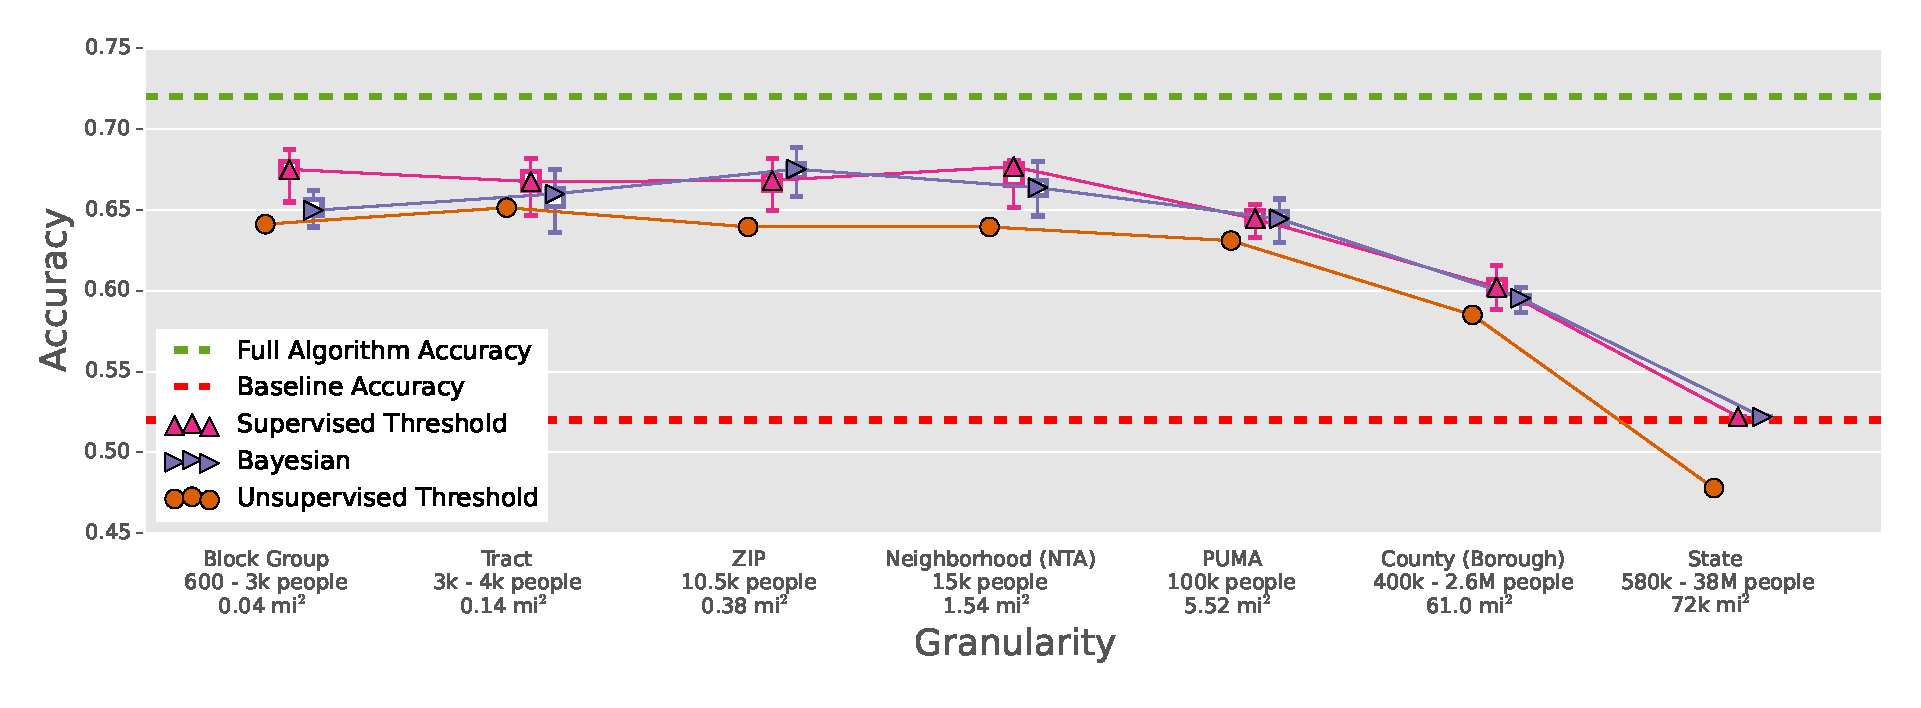
\includegraphics[width=\textwidth]{fig/granularity_plot_both_baselines.eps}
    \caption{Accuracy of ethnicity prediction versus granularity for our NY population using several different inference techniques. Accuracy increases slightly at the ZIP code and neighborhood granularities and then decreases. Interestingly, the Bayesian algorithm, which uses only counts of visits to locations, performs comparably to the Supervised Threshold algorithm, which uses data on the ethnicity of visited locations.}
    \label{fig:big_plot}
\end{figure*}

A detailed comparison of accuracy as a function of granularity and inference scenario can be seen in Figure~\ref{fig:big_plot}.
Granularity decreases (each location is a larger geographic area) as the X axis increases, and the Y axis corresponds to accuracy.
The color of each line corresponds to a different inference scenario.
The \textbf{Bayesian} algorithm uses just the counts of location visits as features.
This corresponds to a scenario where labels are available but locations are anonymized.
The \textbf{Unsupervised Threshold} algorithm uses \emph{no} labels, but rather averages the percentage of Caucasians (or men/women) living all locations that a user visits, outputting a label based on if this average is below or above the city's mean.
This corresponds to a problem scenario where locations are known but users are not labeled.
% To test if labeled data was necessary to guess ethnicity, we developed a simple decision rule that used no labels. Based on Census data we calculated the average percentage of Caucasians living in all locations that a user visited. If this percentage was over the metropolitan area's average, we predicted that the user was Caucasian. If it was below, we predicted that the user was of a minority ethnicity.
% We called this the \textbf{Unsupervised Threshold} algorithm.
In comparison, the \textbf{Supervised Threshold} algorithm learns a threshold via the labeled data, rather than using the city's mean, corresponding to a scenario where there are some labeled users and ``raw" or lightly anonymized location data that can be linked to the census.
% We compared this algorithm to an algorithm with access to labeled data, which learned an optimal threshold rather than using one derived from publicly available Census data and which we dubbed the \textbf{Supervised Threshold} algorithm.
The dashed lines in the graph correspond to our best performing algorithm and the basline.
% Finally, we compared these algorithms against our best performing algorithm, run with all features at the lowest granularity. We call this the \textbf{Full} algorithm.

A few interesting results can be derived from Figure~\ref{fig:big_plot}.
Unsurprisingly, the performance of all algorithms decreases at the most coarse granularities. 
However, the performance stays remarkably flat up to fairly large granularities, without a significant drop until after the PUMA level of roughly 100,000 people.
Additionally, the performance of the Unsupervised Threshold algorithm, which uses \emph{no} labels, is not far from the other algorihtms.
% This is most likely because the ethnicity distributions of larger regions are closer to the overall distribution of the metropolitan area and provide less information. 
Several algorithms improve in performance at medium granularities, such as ZIP and neighborhood, most likely due to the sparsity of our dataset at the most detailed granularity levels.

% This affected our methodology in a few key ways.
% First, we utilized well-understood, commonly-applied techniques that could easily be employed by anyone with access to mobility data.
% We also used publicly available data-sources. 
% Second, to make our results applicable to other sources of location data beyond Instagram, we did not use features specific to Instagram, such as the social network graph or user-generated descriptions.
% Thus, our work should be viewed as a lower-bound on the accuracy of what can be inferred using location data. 
% Adversaries with access to more detailed auxiliary information, more data about each user (such as a contact list or recent purchases), or more advanced machine learning techniques might achieve better results.

% We considered two questions: (1) Can minorities be distinguished from Caucasians? (2) Can women be distinguished from men?
% We represented users as feature vectors, using three classes of features:
% \textbf{geographic} features, such as counts or percentages of visits to locations; 
% \textbf{semantic} features derived from Foursquare, such as the popularity of visited venues or counts of visits to venues with certain categories like ``Restaurant" or ``Park" (the collection of which we explained in \S\ref{sec:method}); 
% and \textbf{Census} derived features, such as the average ethnic makeup of all visited locations or the ethnic makeup of a user's most-visited location.

% We performed all our experiments using the scikit-learn library~\cite{scikit-learn} and tested the algorithms logistic regression, decision trees, naive Bayes, and support vector machines (SVMs). 
% As a baseline, we predicted ethnicity or gender based on the class distribution, giving us baseline accuracies of 52\% for ethnicity in NY, 50\% for ethnicity in LA, and 53\% for gender in NY. 

% \paragraph{Auxiliary Data}

% Auxiliary information about a location derived from Foursquare or the Census may not always be available, e.g., in countries without publicly available census data or when locations are anonymized. 
% Furthermore, a labeled training set of user data may not always be available either. 
% To understand the performance of an algorithm that does not have access to any data beyond counts of visits to locations, we applied our \textbf{Bayesian} algorithm to our data.
% To test if labeled data was necessary to guess ethnicity, we developed a simple decision rule that used no labels. Based on Census data we calculated the average percentage of Caucasians living in all locations that a user visited. If this percentage was over the metropolitan area's average, we predicted that the user was Caucasian. If it was below, we predicted that the user was of a minority ethnicity.
% We called this the \textbf{Unsupervised Threshold} algorithm.
% We compared this algorithm to an algorithm with access to labeled data, which learned an optimal threshold rather than using one derived from publicly available Census data and which we dubbed the \textbf{Supervised Threshold} algorithm.
% Finally, we compared these algorithms against our best performing algorithm, run with all features at the lowest granularity. We call this the \textbf{Full} algorithm.

% \paragraph{Data Granularity}
% The granularity of location data can vary greatly depending on how it is created. %For example, the GPS in a cell phone may have accuracy up to a few yards, while CDR data may cover several square miles. 
% Previous research has investigated the impact of location granularity on anonymity~\cite{de2013unique, Zang:2011hk}. 
% To investigate the impact of granularity on inferences, we represented our location data at several different granularities defined by the Census ranging from block groups to states.
% %For example, in our supervised threshold algorithm, we might use the average ethnicity of the visited counties, as opposed to visited city blocks.
% The ethnic makeup of a large granularity area, such as a county, will typically be more similar to the overall metropolitan area's ethnic makeup than a small granularity area like a city block. Thus, increasing the granularity should make inferences more difficult.



\paragraph{Impact of Data Quantity and Diversity}
% \paragraph{Data Quantity}
Finally, with four different analyses, we studied the impact of data quantity on prediction accuracy.
We examine algorithm accuracy on users grouped according to their number of geolocated Instagram photos and unique ZIP codes.
Both of these are impacted by choices made by users---users who post more might be inherently easier to identify or predict.
We thus did two more analyses where we sampled locations from a user's full set of checkins.
In the first, we ran the Supervised Threshold algorithm on a user's $k$ most visited locations.
In the second, we ran the Supervised Threshold algorithm on $n$ randomly sampled checkins.
The results of this analysis can be seen in~\fig{fig:howmuchdata2}.


% \begin{wrapfigure}{R}{0.5\textwidth}
% % \begin{figure}[h!]
%   \centering
%   % \includegraphics[width=0.49\linewidth]{fig/checkins_to_accuracy.eps}
%   \includegraphics[width=0.49\linewidth]{fig/footprints/checkins_to_accuracy.eps}
%   % \includegraphics[width=0.49\linewidth]{fig/zips_to_accuracy.eps}
%   \includegraphics[width=0.49\linewidth]{fig/footprints/zips_to_accuracy.eps}
%   \caption{Checkin user activity. Left: accuracy as a function of total number of checkins at ZIP code locations. Right: accuracy as a function of number of checkins at distinct ZIP code locations.}
%     \label{fig:howmuchdata}
% % \end{figure}
% \end{wrapfigure}

\begin{figure*}[t]
  \centering
  \includegraphics[width=0.25\linewidth]{fig/footprints/checkins_to_accuracy.eps}
  % \includegraphics[width=0.49\linewidth]{fig/zips_to_accuracy.eps}
  \includegraphics[width=0.25\linewidth]{fig/footprints/zips_to_accuracy.eps}
  % \includegraphics[width=0.49\linewidth]{fig/rand-to-accuracyTract.eps}
  \includegraphics[width=0.24\linewidth]{fig/footprints/rand-to-accuracyTract.eps}
  % \includegraphics[width=0.49\linewidth]{fig/rand-to-accuracyNeighborhood.eps}
  \includegraphics[width=0.24\linewidth]{fig/footprints/rand-to-accuracyNeighborhood.eps}
  \caption{Impact of location quantity and diversity on accuracy. 
  Y axis is accuracy, x axis is (from left to right): 
    (1) Number of checkins used
    (2) Number of unique ZIP codes visited
    (3) Number randomly selected or Top-K Tracts
    (3) Number randomly selected or Top-K Neighborhoods
  % Accuracy of predicting a user's ethnicity from a small number of locations chosen either as most frequently visited locations or randomly. The algorithm used is the Supervised Threshold algorithm. Left: tract granularity. Right: neighborhood granularity.
  }
    \label{fig:howmuchdata2}
\end{figure*}

% In particular, we investigated to what extent a user's total number of checkins and the geographic diversity of those checkins impacted prediction accuracy. We binned users according to how many checkins they made and how many distinct ZIP codes they visited, and then calculated accuracy for each bin. Again, we used five-fold cross validation and 30 different partitionings. Figure~\ref{fig:howmuchdata} shows these results. We compare our Bayesian approach with the highest-performing ``Full" algorithm.

% \subsection{Results}
% \label{subsec:inference-results}

% The results of our best-performing algorithms are displayed in Table~\ref{tab:all-tasks}, and a detailed comparison of accuracy as a function of granularity can be seen in Figure~\ref{fig:big_plot}.
% Our results suggest that geotag data can be used to infer an individual's ethnicity and gender. The accuracy for predicting ethnicity falls squarely within what has been reported for other types of datasets. On the lower bound, in their work of predicting individual Twitter users as African American or not based on linguistic features of Tweets~\cite{ICWSM112886} report as best performance an F-1 score of 0.66. On the upper bound, for predicting whether the ethnic origin of a phone user is inside or outside the United States based on a rich feature set containing Internet usage, call, text message, and location features ~\cite{AltshulerAFEP12} achieved an F-measure of 0.81 and for gender an F-measure of 0.61. For gender~\cite{Zhong:2015:YYG:2684822.2685287} achieved an F-measure of 0.81 for social network users in Beijing and 0.82 for Shanghai based on spatial, temporal, and location context knowledge. Given that our dataset contains far fewer features our results demonstrate that geotags are surprisingly powerful in predicting gender and ethnicity. 

% \paragraph{Auxiliary Data}

% It can be observed in Figure~\ref{fig:big_plot} that the Supervised Threshold algorithm performs much better than the Unsupervised Threshold algorithm suggesting that labeled data improves the algorithmic accuracy across the board by roughly 5\%. Interestingly, the Bayesian algorithm performs comparably to the Supervised Threshold algorithm. Thus, an algorithm with no semantic information about visited locations performs just as well as one that knows the ethnic makeup of all visited locations. This suggests that an adversary with enough location data labeled with demographic data could obtain reasonable levels of accuracy with no knowledge of what locations were visited. Even if locations are ``anonymized," that is, GPS coordinates or venue names were obscured, they can still be used to infer demographic information about the user.

% Another interesting result is that both our Bayesian algorithm and Uninformed algorithm perform well, with the Uninformed algorithm outperforming the Unsupervised Threshold above the neighborhood granularity and the Bayesian algorithm outperforming the supervised threshold. This means that given enough labeled data of counts of visits to locations, an algorithm with no auxiliary information can infer ethnicity with relative good accuracy.

% \paragraph{Data Granularity}
% \label{subsec:inference-granularity}

    % \item \emph{Bayesian}: We tested the simple-hypothesis testing algorithm described in the previous section, which relies on strong assumptions of human mobility.
    % \item \emph{Foursquare}: We ran logistic regression using only the features derived from Foursquare.
    % \item \emph{Full}: The best performing algorithm from \S\ref{subsec:inference-overall} which uses features derived from geography, the US Census, and Foursquare. This serves as an upper bound on performance.

% The Full algorithm (that is, our best performing algorithm, with access to all features at all levels of granularity) achieves the best performance; no algorithm with access to restricted, coarser-grained features is as accurate.
% Comparing this set with our Unsupervised Threshold algorithm shows that auxiliary information provides a large performance boost. However, interestingly, many of the algorithms which only use counts of visits to areas within NY perform as well as the richer features derived from Foursquare. 

% The performance of all algorithms decreases at the most coarse granularities. This is most likely because the ethnicity distributions of larger regions are closer to the overall distribution of the metropolitan area and provide less information. Several algorithms improve in performance at medium granularities, such as ZIP and neighborhood. This is most likely caused by the sparsity of our dataset at the most detailed granularity as many blocks are only visited by a few users.

% \paragraph{Data Quantity}

% It appears that the accuracy of ethnicity prediction improves with the total number of checkins a user has made as shown in Figure~\ref{fig:howmuchdata}. The distinct number of ZIP checkins of a user provides a separate measure of user activity as a user could have a large fraction of checkins in few ZIP codes. We can observe a substantial boost in accuracy after a user checked in at 12 distinct ZIP codes.



%For the Full algorithm we observe a drop in accuracy after 24 ZIP codes, followed by a steady upward trend. 
% While it can be observed that an increase in accuracy generally correlates with increases in total and distinct numbers of ZIP checkins, those variables seem unable to fully explain it. After all, for LA the accuracy decreases until it reaches 79-159 total ZIPs. For NY, users with zero to seven distinct ZIP codes could be predicted more accurately than those having seven to 29. It appears that some ZIP codes increase prediction accuracy better than others.

% In order to explore the individual ZIPs' predictive power we performed two multiple linear regressions---one for NY and one for LA---with the percentage of a ZIP code's inclusion in correct classifications (i.e., the set of correct classifications in which a ZIP code occurs divided by the set of all classifications in which the ZIP code occurs) as the dependent variable and as independent variables (1) the total number of checkins to a ZIP code, (2) the distinct number of users checking in at a ZIP code, and (3) the percentage of Caucasian/minority checkins to a ZIP code. In our regressions we only included ZIP codes that had checkins from at least five distinct users, which left us with 527 different ZIP codes for NY and 207 for LA. 
% 
% We observed that the percentage of Caucasian/minority visits at a ZIP code correlates statistically significantly ($p<0.05$) to its inclusion in the set of correct classifications. Thus, for example, if we have a ZIP code that has 90\% minority checkins and 10\% Caucasian checkins, it was much more likely part of a successful classification than a ZIP code that has equal percentages of minority and Caucasian checkins. The other variables did not prove to be statistically significant. We also tested minority status as independent variable. However, it does not appear to be easier to predict minorities over Caucasians or vice versa.

% We also found that when a user is only observed in a limited set of locations, the inference accuracy increases fast with a relatively small increase in the number of locations. Moreover, it is not even required to focus on the most significant locations of a user to get good inference accuracy. Observations of a user in a few random locations at the tract or neighborhood level might be enough for predicting ethnicity, and those locations may be even selected randomly and must not be necessarily related to the user's most significant places. These results, which are displayed in Figure~\ref{fig:howmuchdata2}, suggest that inference for the purpose of ethnicity identification is quite robust to data sparseness and obfuscation methods.





% ``particularly, heterogeneity holds only for well-off areas. These areas tend to attract people living in areas of varying deprivation. By contrast, Londoners in well off areas do not tend to visit communities that are deprived.''~\cite{conf/pervasive/LathiaQC12}








% \subsection{Inferring Ethnicity and Gender}
% \label{subsec:inference-overall}

% % (1) Using location data, can we predict a user's ethnicity and gender with accuracy better than a random guess? (2) What is the impact of auxiliary information and the granularity of the location data on this prediction? 

% To determine if we could predict the ethnicity and gender of a user with high accuracy, we represented users as feature vectors and tested a number of commonly used machine learning algorithms. We performed all our experiments using the scikit-learn library~\cite{scikit-learn} and tested the algorithms logistic regression, decision trees, naive Bayes, and support vector machines (SVMs). 
% We attempted to distinguish between men and women and turned the question of ethnicity into a binary classification question between Caucasians and minorities. This yielded roughly equal class sizes.

% We used many features, falling into one of three groups: 
% \textbf{general} location-based features, counts or percent of visits to each location; 
% \textbf{Foursquare}-based features such as the average popularity of visited venues or counts of visits to venues with certain categories (the collection of which were mentioned in \S\ref{sec:method}); 
% and \textbf{Census} derived features such as the average ethnic makeup of all visited locations and the ethnic makeup of a user's most-visited location.   
% For each experiment we applied five-fold cross validation, that is, we broke down our data into five groups, trained on four groups, and tested on the remaining group. After running all algorithms with all features, our best results are reported in Table~\ref{tab:all-tasks}. 


% Our results suggest that geotag data can be used to infer an individual's ethnicity and gender. The accuracy for predicting ethnicity falls squarely within what has been reported for other types of datasets. On the lower bound, in their work of predicting individual Twitter users as African-American or not based on linguistic features of Tweets, ~\cite{ICWSM112886} report as best performance an F-1 score of 0.655. On the upper bound, for predicting whether the ethnic origin of a phone user is inside or outside the United States based on a rich feature set containing Internet usage, call, text message, and location features ~\cite{conf/socialcom/AltshulerAFEP12} achieved an F-measure of 0.806 and for gender an F-measure of 0.611. Given that our dataset contains far fewer features our results demonstrate that geotags are surprisingly powerful in predicting ethnicity and gender. 

% \subsection{The Impact of Granularity and Auxiliary Information}
% \label{subsec:inference-granularity}

% \begin{figure*}[htb!]
%   \centering
%   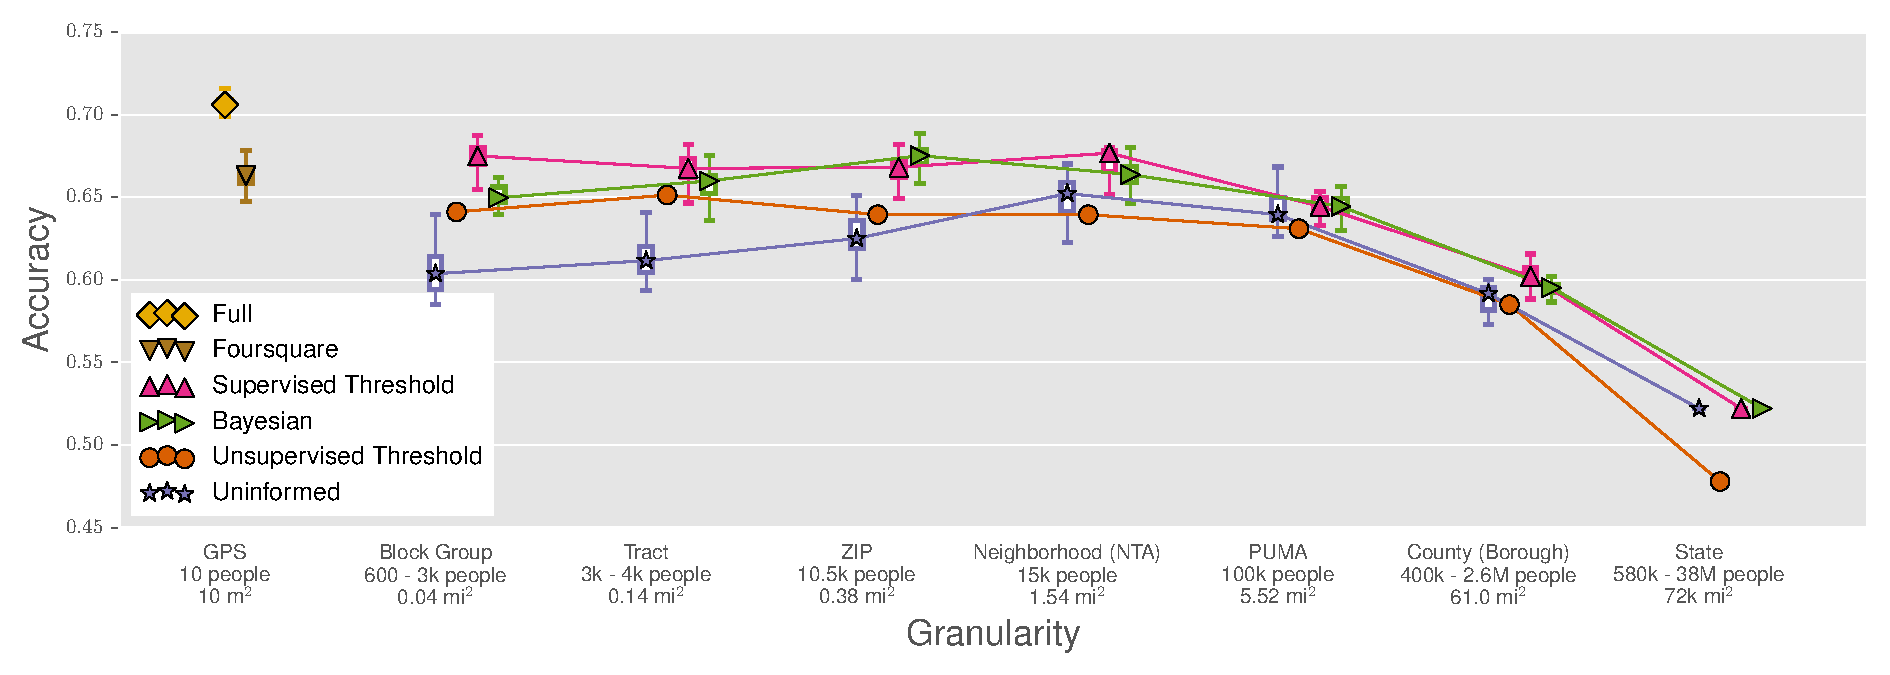
\includegraphics[width=\textwidth]{fig/big_plot_ggplot.pdf}
%   \vspace{0.2ex}
%     \caption{Accuracy of ethnicity prediction versus granularity for our NY population using several different inference techniques. Unsurprisingly, the Full algorithm, which uses features from Foursquare, the US Census, and simple geography, performs the best. Interestingly, however, much simpler algorithms with limited information achieve comparable results.}
%     \label{fig:big_plot}
% \end{figure*}


% Auxiliary information about a location derived from Foursquare or the Census may not always be available, such as in countries without publicly available census data or when locations are anonymized. Additionally, the granularity of location data can vary greatly depending on how it is created. For example, the GPS in a cell phone may have accuracy up to a few yards, while CDR data may cover several square miles. The granularity of location data is often lowered in order to increase the privacy of a dataset. 

% % To study how auxiliary information and granularity impact prediction accuracy we construct feature vectors from the users' sets of visited latitude-longitude locations. We categorize a feature as \emph{informed} if it uses auxiliary information, i.e., census data or Foursquare categories, and as \emph{uninformed} otherwise. In particular, based on census data we computed a threshold by taking the weighted mean of the ethnic distributions for the locations a user visited, and if the user's mean checkin percentage was above the mean for Caucasian visitors, the user was labeled Caucasian and as minority otherwise. Because this method does not require any labeled data, we categorize the resulting features as \emph{unsupervised}. However, other features are \emph{supervised} as they are based on training data labeled by our annotators. 

% In order to understand the impact of auxiliary information and granularity on our ability to make inferences, we compared the highest performing algorithm of \S\ref{subsec:inference-overall} with algorithms that used only a subset of the Foursquare features, Census features, or general features. Additionally, to see if labeled profiles were necessary to infer ethnicity, we tested simple decision rules that required no training.
% % Using different combinations we investigate the following feature sets:
% We employed the following algorithms:

% \begin{itemize}
%     % uninformed supervised features without any auxillary information trained on the percentages of checkins at the various locations.
%     \item \emph{Unsupervised Threshold}: To test if labeled data was necessary to guess ethnicity, we developed a simple decision rule that used no labels. Using census data, we calculated the average percentage of Caucasian people living in all locations that a user visited. If this percentage was over the city's average, we predicted that the user was Caucasian. If it was under, we predicted that the user was a minority.
%     \item \emph{Supervised Threshold}: As a point of comparison, we ran the previously-mentioned decision rule but this time learned the threshold on a set of training data. The performance of this relative to the unsupervised threshold algorithm shows the impact of labeled data.
%     \item \emph{Uninformed}: We ran our best performing algorithm (logistic regression) on a reduced feature set of only the percentages of a user's checkins at each location. This serves as a lower bound on the performance of an algorithm on labeled data using only location information.
%     \item \emph{Bayesian}: We tested the simple-hypothesis testing algorithm described in the previous section, which relies on strong assumptions of human mobility.
%     \item \emph{Foursquare}: We ran logistic regression using only the features derived from Foursquare.
%     \item \emph{Full}: The best performing algorithm from \S\ref{subsec:inference-overall} which uses features derived from geography, the US Census, and Foursquare. This serves as an upper bound on performance.
% \end{itemize}

% We also wanted to understand the impact of location granularity on prediction accuracy. We thus represented our location data at several different granularities defined by the U.S. Census, ranging from block groups to states.
% % , as displayed on the X axis of Figure~\ref{fig:big_plot}.
%  % (600-3,000 individuals) to county (400K- 2.6 million individuals) and state (580K-38 million individuals). 
%  We additionally considered GPS granularity.
%   % (10 individuals).

% For all applicable algorithms, we again employed five-fold cross validation. To view the stability of our algorithms we repeated this process 30 times, using 30 different data partitionings into training and test sets. We ran all algorithms on our dataset of New York City based users.
% The results of this experiment are shown in Figure~\ref{fig:big_plot}.


% % \paragraph{The Impact of Auxillary Information} 
% % \paragraph{The Impact of Granularity}

% It can be observed that the Full algorithm achieves the best performance, as might be expected. Comparing this set with our Uninformed set shows that auxiliary information provides a large performance boost. However, interestingly, many of the algorithms which only use counts of visits to areas within NY perform as well as the richer features derived from Foursquare. Another interesting result is that both our Bayesian algorithm and Uninformed algorithm perform well, with the Uninformed algorithm outperforming the Unsupervised Threshold above the neighborhood granularity and the Bayesian algorithm outperforming the supervised threshold. This means that given enough labeled data of counts of visits to locations, an algorithm with no auxiliary information can infer ethnicity with relative good accuracy.

% The performance of all algorithms decreases at the largest granularities. This is most likely because the ethnicity distributions of larger regions are closer to the overall city distribution and provide less information. Several algorithms improve in performance at medium granularities such as ZIP and Neighborhood. This is most likely caused by the sparsity of our dataset at the highest granularity, as many blocks are visited by only a few users.

% \subsection{The Impact of User Activity}
% \label{sec:user-activity}

% % Finally, we also studied the impact of user activity on prediction accuracy. In particular, we investigated to what extent a user's total number of checkins and the geographic diversity of those checkins impacted prediction accuracy. We binned users according to how many checkins they made and how many distinct ZIP codes they visited, and then calculated accuracy for each bin. Again, we used five-fold cross validation and 30 different partitionings. Figure~\ref{fig:howmuchdata} shows these results. We compare our Bayesian approach with the highest-performing ``Full" algorithm.

% It appears that the accuracy of ethnicity prediction improves with the total number of checkins a user has made. The distinct number of ZIP checkins of a user provides a separate measure of user activity as a user could have a large fraction of checkins in few ZIPs. We can observe a substantial boost in accuracy after a user checked in at 12 distinct ZIP codes. For the Full algorithm we observe a drop in accuracy after 24 ZIP codes, followed by a steady upward trend. 
% % While it can be observed that an increase in accuracy generally correlates with increases in total and distinct numbers of ZIP checkins, those variables seem unable to fully explain it. After all, for LA the accuracy decreases until it reaches 79-159 total ZIPs. For NY, users with zero to seven distinct ZIP codes could be predicted more accurately than those having seven to 29. It appears that some ZIP codes increase prediction accuracy better than others.

% In order to explore the individual ZIPs' predictive power we performed two multiple linear regressions---one for NY and one for LA---with the percentage of a ZIP code's inclusion in correct classifications (i.e., the set of correct classifications in which a ZIP code occurs divided by the set of all classifications in which the ZIP code occurs) as the dependent variable and as independent variables (1) the total number of checkins to a ZIP code, (2) the distinct number of users checking in at a ZIP code, and (3) the percentage of Caucasian/minority checkins to a ZIP code. In our regressions we only included ZIP codes that had checkins from at least five distinct users, which left us with 527 different ZIP codes for NY and 207 for LA. 

% We observed that the percentage of Caucasian/minority visits at a ZIP code correlates statistically significantly ($p<0.05$) to its inclusion in the set of correct classifications. Thus, for example, if we have a ZIP code that has 90\% minority checkins and 10\% Caucasian checkins, it was much more likely part of a successful classification than a ZIP code that has equal percentages of minority and Caucasian checkins. The other variables did not prove to be statistically significant. We also tested minority status as independent variable. However, it does not appear to be easier to predict minorities over Caucasians or vice versa.


% \begin{figure}[h]
%   \centering
%   \includegraphics[width=0.49\linewidth]{fig/checkins_to_accuracy.eps}
%   \includegraphics[width=0.49\linewidth]{fig/zips_to_accuracy.eps}
%   \caption{Checkin user activity. Left: accuracy as a function of total number of checkins at ZIP code locations. Right: accuracy as a function of number of checkins at distinct ZIP code locations.}
%     \label{fig:howmuchdata}
% \end{figure}


% \begin{figure}[h]
%   \centering
%   \includegraphics[width=0.49\linewidth]{fig/rand-to-accuracyTract.eps}
%   \includegraphics[width=0.49\linewidth]{fig/rand-to-accuracyNeighborhood.eps}
%   \caption{}
%     \label{fig:howmuchdata2}
% \end{figure}


% % ``particularly, heterogeneity holds only for well-off areas. These areas tend to attract people living in areas of varying deprivation. By contrast, Londoners in well off areas do not tend to visit communities that are deprived.''~\cite{conf/pervasive/LathiaQC12}

% \section{Conclusion}
% \label{sec:conclusion}
% Location data is increasingly available and its use holds many risks and opportunities.
This study highlights the risks and opportunities of discriminative big data analysis by demonstrating that it is possible to infer Internet users' ethnicities and genders based on location data \emph{alone}. It also shows that mobility patterns can be studied using publicly available data. Internet users may often be unaware that releasing such data could also disclose possibly sensitive personal information. Simply reducing granularity proved to be insufficient to prevent such privacy leakage as mobility remains discriminative. However, the trove of geotagged pictures available through individual online profiles also yields important insights for beneficial uses, for example, by city planners and social scientists. 

As our dataset is similar, both demographically and mobility-wise, to other datasets as shown in \S\ref{sec:patterns}, we believe that our results are generalizable and applicable to other unlabeled datasets. Although it could be claimed that our data is biased by the fact that the users in our study have willingly disclosed their gender and ethnicity by publicly using Instagram, we want to stress that it would be difficult and possibly unethical to create a labeled dataset of users who \emph{do not} want to disclose their gender and ethnicity.

This work motivates multiple avenues of further research: First, it enables the extension of demographic mobility analysis to many researchers using shareable public datasets and reproducible results. Beyond ethnicity and gender, attributes such as age, occupation, and other lifestyle features may be extracted from users' pictures, and naturally there are many other mobility properties to account for beyond, for example, daily ranges. Second, better understanding the discriminative power of location data might inform the design of tools for raising user awareness about the information they reveal. This insight motivates revisiting mobility modeling and the inferences it renders possible to empower users to make at will their locations as clear as a photograph or as opaque as footprints in the mud. 

% , showing also the impact of granularity, location anonymization, and data quantity on this inference.
% Additionally, we show statistically significant differences in mobility at a population level between gender and ethnic groups.
% We first demonstrated that geotag data from Instagram reproduces and accurately represents both mobility behaviors from a prior study and demographic patterns from the U.S. Census.
% We hope that our methodology will be useful for others hoping to obtain location data labeled with demographic information.
% All data used in the study will be made available in an anonymized fashion upon publication.

% New m

% Location data is increasingly available and its use holds many risks and opportunities.
% As smartphones become more affordable and ubiquitous, more people will be regularly 
% % As we've shown, 
% They may not realize that releasing location data can also reveal information about their gender and ethnicity



\subsubsection{Scaling up the Census with Social Media}

% \begin{abstract}
The growth of publicly available online information from social networks provides many opportunities to demographic researchers.
However, this data is often messy and unlabeled, causing researchers to need to label profiles with demographics.
This labelling is either done manually, a costly and time-consuming process, or done via automated algorithms.
The inputs to these algorithms have previously been text-based, taking a user's posts or name as input.
Techniques involving computational vision have been left unused, due to a lack of training data from users and problems of low accuracy.

In this work, we evaluate the feasibility of combining modern facial recognition techniques with publicly available social media images to conduct large scale demographic research.
We find that facial recognition can be used to label the gender and race of social media profiles with high precision and recall.
We further investigate factors that improve or hinder demographic labeling accuracy, showing a disparity between the accuracy of labelings of profiles of racial majority and minorities.
We conclude with ideas for future improvements and research.
% \end{abstract}


\textbf{Introduction} \\
The great wealth of publicly available, online social networking data has been a boon to demographic research due to its richness and scale.
Never before has such an amount of human behavioral data been easily obtained and analyzed.
However, before this data can be used to study demographics, each user must be labeled with demographic categorizations. 
This poses a particular challenge in many online social networking (OSN) sites which often do not display or even obtain the demographic information of its users.

To meet this need, researchers in the past have tried a variety of techniques.
Manual labeling by individually investigating each profile is costly in terms of time, effort, and money.
Some studies have relied on data provided by marketing companies or data aggregators~\cite{Goel:2012ut, biinferring}.
Due to cost and issues of reproducibility, these sources of data are not available to all researchers.

To improve the scale of labeling while keeping costs low, researchers have used automated techniques which range in complexity.
For example, researchers have compared public names to lists of gender and ethnicity for those names~\cite{mislove-2011-twitter, ICWSM101534}.
Others have run simple algorithms on location data~\cite{riederer2015cosn} or more sophisticated techniques that incorporate text posted and the structure of a user's social network~\cite{ICWSM112886, pennacchiotti2011democrats}.
These techniques offer some promise but often are not very robust and may not be applicable to OSNs with little textual interaction, such as Instagram.

% TODO: This doesn't really fit.
Researchers that use these automated tools for labeling must be wary of introducing algorithmic bias.
As argued in~\cite{Selbst:2014wi}, data mining can lead to biased results.
Algorithms that have disparate accuracies in demographic labeling could cause erroneous or biased results.

In the past, computational vision has not been an effective technique for labeling the demographics of social media users, due to three issues: (1) CV algorithms being too slow, (2) CV algorithms having low accuracy, (3) a lack of publicly available and uniformly popular photographs as data.
However, in recent years, face recognition tools have improved to become both highly accurate and efficient.
Additionally, the social network Instagram has made image-sharing a ubiquitous activity across most of the developed and much of the developing world.

Instagram is an interesting social network to study for a variety of reasons.
With over 400 million users at the time of writing, over 5\% of the world's population user Instagram.
A quarter of these users are based inside the United States, meaning that nearly 1 in 3 United States citizens uses Instagram~\cite{igstats}.
Beyond its scale, Instagram is interesting for its content.
Photographs are extremely rich, capturing information on all sorts of human activities and interactions.
Although images can be more difficult to analyze than text, the research community has begun to study Instagram behavior~\cite{hu2014we, bakhshi2014faces} and even selifes~\cite{souza2015dawn}.

In this paper, we show that a popular face recognition API can be used to scalably and accurately learn the gender and race of Instagram users.
We use a dataset of 200 Instagram profiles, labeled for gender and race, to analyze the practicality and accuracy of facial recognition, achieveing 86\% accuracy for gender and 82\% accuracy for race in a limited setting.
We additionally explore the accuracy of labeling different demographics as the amount of data increases, showing some concerns about algorithmic bias.
We conclude with ideas for future work.

\textbf{Data} \\
\textbf{Collection} \\
We used a subset of the Instagram data collected in~\cite{riederer2015cosn}.
In this paper, the authors gathered the metadata (such as time of photo, URL of image, tags, location, etc.) for all photographs of a ``root" user, Kevin Systrom, the founder of Instagram.
They then collected the user IDs of users who had commented or liked his photos, gathered their metadata, and repeated this process.
A subset of these users were then selected based on geography-- only users with more than half of their photographs taken in Los Angeles or New York were kept.

Two research assistants labeled a randomly selected subset of 200 of these profiles for gender and race.
After filtering for private, deleted, or business profiles, 172 profiles remained.
For gender, the labelers selected from male, female, or other.
In practice, only the male or female categories ended up being used.
For race, a subset of the United States Census categories were used: White, Black, Hispanic, Asian, and other.
The labelers agreed on gender for 170 of the profiles and for race on 147.
The process resulted in 76 profiles as Male and 94 as Female.
For race, 75 were labeled White, 28 as Hispanic, 27 as Black, 16 as Asian, and 1 as other.

Our next step was to recognize and label faces present in these Instagram users' profiles using computer vision.
For this task, we used Face++~\cite{faceplusplus}, a popular API with reported high degress of accuracy~\cite{bakhshi2014faces}.
In addition to recognizing faces within images, Face++ labels race from {White, Black, Asian} with a \emph{confidence score} 0-100, gender from {Male, Female} with a \emph{confidence score} 0-100.

For each user in this data set, we gathered the metadata of the first 100 Instagram photos.
Each image was then analyzed with the Face++ API.
Face++ only requires that a URL to an image is passed to it.
Therefore, this methodology does \emph{not} require that any images are downloaded, uploaded, or even viewed by a human labeler.
Note that not every photo on Instagram has a face in it, and some have more than one.

This resulted in 170 distinct users with at least one or more face present in their photos.
We obtained 5,272 photos and depicting 12,143 faces. 
Additionally, for each user, we passed the URLs for their profile pictures.
A total of 70 users had profile pictures in which Face++ could detect a face.
73 faces were found: 2 profiles pictures had 2 faces in them.

\textbf{Description}


\begin{figure}[t]
  \centering
  \begin{subfigure}[b]{.21\textwidth}
    \centering
    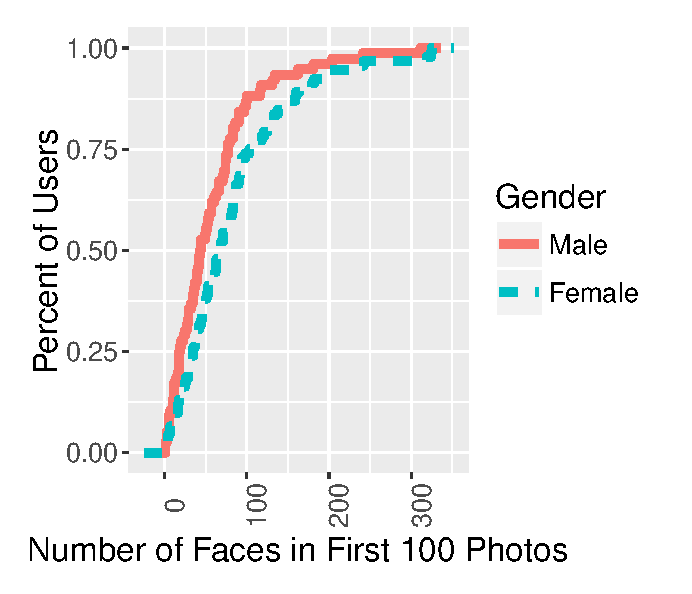
\includegraphics[width=\linewidth]{fig/census/face_cdf_gender.eps}
    \caption{}
    \label{fig:face_cdf_gender}
  \end{subfigure}
  \begin{subfigure}[b]{.21\textwidth}
    \centering
    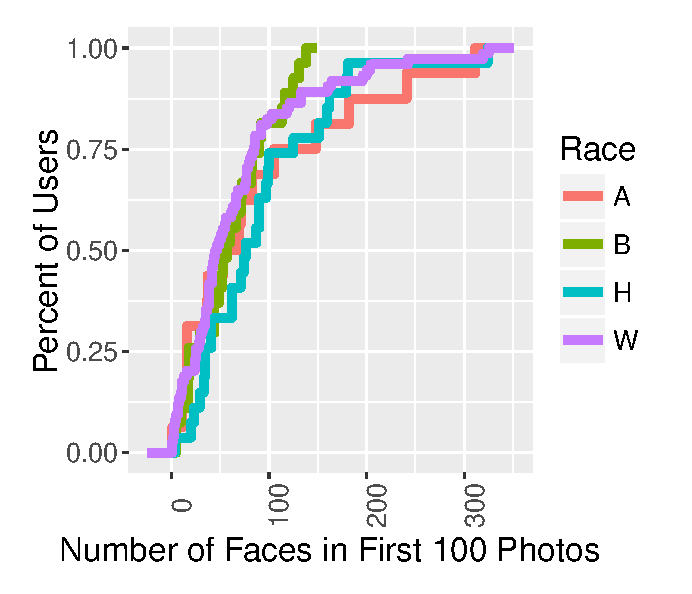
\includegraphics[width=\linewidth]{fig/census/face_cdf_race.eps}
    \caption{}
    \label{fig:face_cdf_race}
  \end{subfigure}
  \caption{}
  \label{fig:face_cdf}
\end{figure}

\begin{figure}[t]
  \centering
  \begin{subfigure}[b]{.21\textwidth}
    \centering
    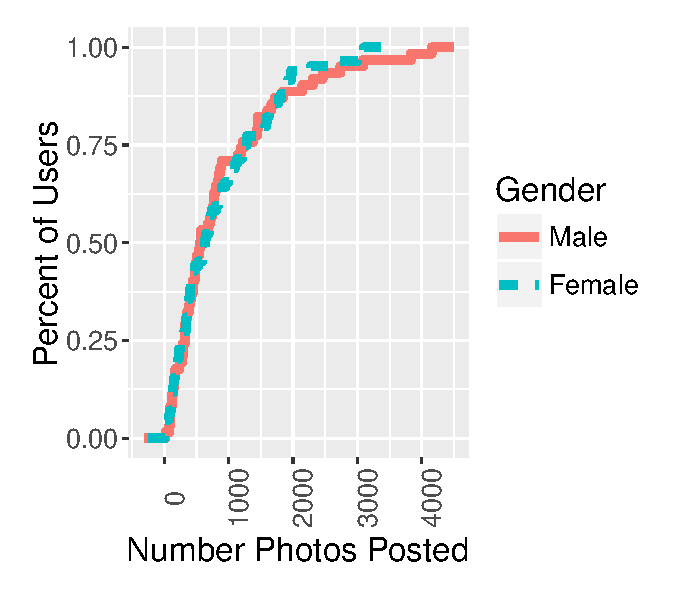
\includegraphics[width=\linewidth]{fig/census/numphoto_cdf_gender.eps}
    \caption{}
    \label{fig:numphoto_cdf_gender}
  \end{subfigure}
  \begin{subfigure}[b]{.21\textwidth}
    \centering
    \includegraphics[width=\linewidth]{fig/census/numphoto_cdf_race.eps}
    \caption{}
    \label{fig:numphoto_cdf_race}
  \end{subfigure}
  \caption{}
  \label{fig:numphoto_cdf}
\end{figure}


\begin{figure}[t]
  \centering
  \begin{subfigure}[b]{.21\textwidth}
    \centering
    \includegraphics[width=\linewidth]{fig/census/followers_cdf_gender.eps}
    \caption{}
    \label{fig:followers_cdf_gender}
  \end{subfigure}
  \begin{subfigure}[b]{.21\textwidth}
    \centering
    \includegraphics[width=\linewidth]{fig/census/followers_cdf_race.eps}
    \caption{}
    \label{fig:followers_cdf_race}
  \end{subfigure}

  \begin{subfigure}[b]{.21\textwidth}
    \centering
    \includegraphics[width=\linewidth]{fig/census/following_cdf_gender.eps}
    \caption{}
    \label{fig:following_cdf_gender}
  \end{subfigure}
  \begin{subfigure}[b]{.21\textwidth}
    \centering
    \includegraphics[width=\linewidth]{fig/census/following_cdf_race.eps}
    \caption{}
    \label{fig:following_cdf_race}
  \end{subfigure}
  \caption{}
  \label{fig:follow_cdf}
\end{figure}

We next compared several Instagram behaviors by demographic.
Figure~\ref{fig:face_cdf_gender} shows that women in our dataset typically have more faces in their photographs than men.
There appears to be more parity in number of faces for each of the considered racial groups, with Hispanics and Asians displaying slightly more faces in their photos.

We examine potential differences in the total number of photos posted by a user to their account in Figure~\ref{fig:numphoto_cdf}.
There does not appear to be a great difference for any particular group.

We investigate the relationship between gender, race, and following behavior in Figure~\ref{fig:follow_cdf} .
Instagram has a directional follower relationship, akin to that of Twitter.
If a user, Alice, follows Bob, it means that Alice will see updates from Bob in her feed.
Bob, however, will not see updates from Alice unless he decides to follow her.
Figures~\ref{fig:followers_cdf_gender} and~\ref{fig:following_cdf_gender} show differences in following behavior within our dataset for gender. 
It appears that men have more followers, and follow slightly more people.

In Figures~\ref{fig:followers_cdf_race} and~\ref{fig:following_cdf_race}, we see can make a few observations for following behavior among race in our dataset.
First, we see that the upper 50\% of Black users in our dataset have more followers than other groups, except for at the very top percentiles, where White users dominate.
At the highest percentiles, Black users \emph{follow} the most people.
% TODO: mention Black Twitter...
% http://www.slate.com/articles/technology/technology/2010/08/how_black_people_use_twitter.html
% Maybe http://dl.acm.org/citation.cfm?id=1963503
% duggan and smith: demo of key social networking platforms



\textbf{Methodology}
% Recognizing and labeling the faces present in each photo does not definitively tell us the gender or race of the user profile. 
The face recognition software only works at the level of a single photograph.
% This does not tell us the race or gender of the user on which these photographs appear.
We thus need to use an algorithm to go from the data of each picture to labeling an entire profile.
We rely on one main assumption: the owner of profile will appear in more photos than any other individual.

This assumption led us to test several different algorithms: 
\begin{itemize}
\item \textbf{Majority rule}: Count each face as a vote. 
  Profile is labeled with the gender (or race) with the most votes.
\item \textbf{Weighted majority rule}: Count each face as a vote.
  However, a face now gets as many votes as the confidence score.
  Thus, faces with lower confidence get lower weight.
  Profile is labeled with the gender (or race) with the most votes.
\item \textbf{Profile picture}: We simply take the result of the profile picture labeling.
\end{itemize}

Additionally, we applied a ``face weight" correction to all of these.
In a photo with three faces, only one of these faces could be the user.
It therefore might make sense to weight each face in this photo lower than in a photo with one face.
The face weight (fw) correction does just this, multiplying the weight of photo by the inverse of the number of faces in that photograph.
In our original example, the weight of each of the three faces would be multiplied by one third.
This is equivalent to averaging the gender or race (potentially with confidence scores) of all users in a photograph.


\textbf{Results}

\textbf{Gender}
Our human labelers categorized 76 profiles as Male and 94 as Female.
Running our three algorithms with and without the face weight correction, we obtained the following results:
\begin{itemize}
\item \textbf{Majority rule}: 85.1\%
\item \textbf{Weighted majority rule}: 85.7\%
\item \textbf{Majority Rule, FW}: 86.9\%
\item \textbf{Weighted Majority Rule, FW}: 87.5\%
\item \textbf{Profile picture}: 86.3\%
\end{itemize}

We observe that using the face weight correction improves the results for both algorithms.
Although profile pictures provide accurate information, only 70 out of 170 of these users had a profile picture that included a face.
For the remainder of this section, we will focus on the highest accuracy algorithm, weighted majority rule with FW.
A feature of this algorithm is that it outputs a probability for each user, enabling us to analyze the performance in more detail.
% \begin{figure}[!tbp]
%   \centering
%   \begin{minipage}[b]{0.4\textwidth}
%     \includegraphics[width=\textwidth]{flower1.jpg}
%     \caption{Flower one.}
%   \end{minipage}
%   \hfill
%   \begin{minipage}[b]{0.4\textwidth}
%     \includegraphics[width=\textwidth]{flower2.jpg}
%     \caption{Flower two.}
%   \end{minipage}
% \end{figure}

\begin{figure}[h]
  \centering
  \begin{minipage}{.21\textwidth}
    \centering
    \includegraphics[width=\linewidth]{fig/census/accuracy_gender.eps}
    \caption{Predicted accuracy versus actual accuracy }
    \label{fig:accuracy_gender}
  \end{minipage}
  \begin{minipage}{.21\textwidth}
    \centering
    \includegraphics[width=\linewidth]{fig/census/roc_gender.eps}
    \caption{True positive versus false positive rate when labeling at various threshold levels.}
    \label{fig:roc_gender}
  \end{minipage}
  \caption{}
  \label{fig:accuracy_gender_all}
\end{figure}

\begin{figure}[h]
  \centering
  \includegraphics[width=.5\linewidth]{fig/census/facebin_gender.eps}
  \caption{Number of faces detected in first 100 photos vs. accuracy, by gender}
  \label{fig:facebin_gender}
\end{figure}
% TODO: add the boxplot thing in here, just because this looks bad right now

In Fig.~\ref{fig:accuracy_gender}, we group individuals on how what our algorithm predicts is the likelihood that that individual is female, and plot the accuracy within each group.
This shows us how well calibrated our algorithm is; if the output probability estimates are perfectly accurate, then half of the users with estimate 50\% should be female, and this plot should align on the 1:1 line.
Instead, we see that the line is above the diagonal, meaning our accuracy estimate is actually an underestimate.
Most likely, we could incorporate a prior probability into our algorithm to make it better calibrated.

In Fig.~\ref{fig:roc_gender}, we plot an ROC curve, showing the trade-off between accurate and inaccurate labelings when using a threshold on the algorithm's output probability.
For example, if we label as female all users with a probability of female over 60\%, around 75\% of female users would be correctly labeled, and we would exclude properly all but around 7\% of males.

In Fig.~\ref{fig:facebin_gender}, we observe that for users labeled female, as more faces are detected in their profiles, accuracy increases.
Perhaps counterintuitively, we see a dip for men, where male users with the 40-80\% most faces have much lower accuracy those in the bottom two quintiles, the bottom 40\%.
One possible hypothesis to explain this is that as some users add more faces, they will start to add a larger diversity of faces.
When this diversity increases, accuracy may decrease.
We leave the question of whether this is the mechanism open for later work.


\textbf{Race} \\

For race, 75 users were labeled White, 28 as Hispanic, 27 as Black, 16 as Asian, and 1 as other.
However, Face++ only labels users as Asian, Black, or White and will therefore always be incorrect on any of our users categorized as Hispanic or ``Other".
Thus, we'll present results both for all users, and for the reduced set of users labeled manually by our research assistants as Asian, Black, or White (``filtered").
Running our algorithms with and without the face weight correction, we obtained the following results:
\begin{itemize}
\item \textbf{Majority rule}: 64.4\% (all) 79.3\% (filtered)
\item \textbf{Weighted majority rule}: 66.2\% (all) 82.1\% (filtered)
\item \textbf{Majority Rule, FW}: 66.4\% 82.2\% (filtered)
\item \textbf{Weighted Majority Rule, FW}: 66.2\% (all), 82.1\% (filtered)
\item \textbf{Profile picture}: 57.1\% (all), 71.1\% (filtered)
\end{itemize}

On the users for which we have some hope of accuracy, the best algorithm achieves 82.2\% accuracy.
For the remainder of this section, we will constrain our results to the Weighted Majority algorithm, FW, due to the probabilities that it outputs and its nearly identital performance to the next best algorithm.
Additionally, we will look at some labelings as a binary classification problem between White users and Minority users.

% TODO: fix titles here
\begin{figure}[h]
  \centering
  \begin{minipage}{.21\textwidth}
    \centering
    \includegraphics[width=\linewidth]{fig/census/accuracy_race_all.eps}
    % \caption{Predicted accuracy versus actual accuracy }
    \label{fig:accuracy_race_all}
  \end{minipage}
  \begin{minipage}{.21\textwidth}
    \centering
    \includegraphics[width=\linewidth]{fig/census/accuracy_race_filtered.eps}
    % \caption{True positive versus false positive rate when labeling at various threshold levels.}
    \label{fig:accuracy_race_filtered}
  \end{minipage}
  % \caption{}
  \label{fig:accuracy_race}
\end{figure}

\begin{figure}[h]
  \centering
  \begin{minipage}{.21\textwidth}
    \centering
    \includegraphics[width=\linewidth]{fig/census/roc_race.eps}
    % \caption{Predicted accuracy versus actual accuracy }
    \label{fig:roc_race}
  \end{minipage}
  \begin{minipage}{.21\textwidth}
    \centering
    \includegraphics[width=\linewidth]{fig/census/facebin_race_filtered.eps}
    % \caption{True positive versus false positive rate when labeling at various threshold levels.}
    \label{fig:facebin_race_filtered}
  \end{minipage}
  \caption{}
  \label{fig:more_race}
\end{figure}

Based on Fig.~\ref{fig:accuracy_race}, the algorithm does not appear to be well-calibrated, both in being overconfident in the users with low probability estimations, and being underconfident in users with higher estimates.

An important aspect of demographic labeling is considering issues of the digital divide or disparate impact.
In Fig.~\ref{fig:more_race}, we see that accuracy is much lower on minorities than it is on White users.
Again, we see a lowering of accuracy as the number of faces increases, akin to the dip in accuracy Male users show in Fig.~\ref{fig:facebin_gender}.

\textbf{Discussion} \\
Among our dataset, we see some examples of differences in behavior.
For example, women tended to have more faces in their photos, and black users tended to have more followers.
A larger sample and careful statistical analysis should be taken to verify these results.
Applying machine learning to many more profiles could reveal, and possibly help explain, these and other differences in behaviors on Instagram.

In applying these techniques there are dangers of algorithmic bias.
The large difference in accuracy between white users and minority users is an example of this.
Our technique as it stands could suffer from this issue.
For example, users with more diverse faces in their profile (both gender and racially) may be harder to label.
Using a thresholding technique to only obtian high-accuracy users might leave only users who display strong homophily.

Further exascerbating the problem is that racial minority users actually \emph{decrease} in accuracy as there is more data about them, up to a certain point. 
Clearly more work is need to be done to understand this issue.
It may be important to consider the trade-offs here.
A more accurate algorithm may not be preferable to an algorithm that is equally accurate across demographic groups, and that behaves similarly in regards to the scaling of data.

% \section{Conclusion}
\textbf{Conclusion} \\
In this work, we've shown that computational vision techniques have some promise in becoming a valuable tool for demographers.
By combining facial recognition with the OSN Instagram, we've proven that the race and gender of users can be inferred with high precision and recall.

We see several important next steps to this work.
First, a larger scale verification of the results of this work should be obtained, with more users, aiming for diversity in many senses-- culturally, economically, racially, geographically, etc.
Such a verification should investigate the accuracy of the technique on various demographics in order to minimize algorithmic bias. 

Another direction is to use more powerful machine learning techniques on this problem.
For example, instead of naively incorporating all faces in a profile, a researcher could cluster faces based on a similarity score.
The largest cluster would most likely contain the users face.
Other facial recognition software packages, with a wider range of races, or with other features, could improve upon these results.

Finally, this technique could be used to engage in studies of various demographic groups and answer different questions.
Do different demographics use social networks in different ways?
What can we learn about interactiokn on the OSN between groups?
Combining demographic data with location data, we could additionally learn about immigration or human mobility.



\section{Proposal Topic I}
\label{sec:proposal-i}
% Algorithmic bias is bad
% Recent work has been more about theory, less about real data analysis
% I have a cool new dataset that allows me to do data analysis

As described in \chap{chap:bias}, an important challenge facing the computer science community is algorithmic bias.
In recent years, an emerging body of work has focused on different mitigating techniques, 
  such as automated discovery of bias, ``de-biasing" existing algorithms, or theoretical analyses of different types of bias.
De-biasing techniques are sure to incur a cost: the objective function of the algorithm is no longer as straightforward, and organizationally new infrastructure needs to be put into place for something that could hurt revenue.
Understanding the key trade-offs between revenue and uncertain risk will be important to insure real-world adoption.
Although there have been some good initial insights, the community has lacked strong data-driven analysis on this trade off.

I propose to fill this gap by applying proposed techniques to real-world problems through the use of an innovative dataset.
Namely, I will look at the real-world problems of recommendation systems within a large social network, focusing on location-based advertising.
As locations are an important signal in user intent and demographics, they are a useful system for advertising.
By the same token, since locations are tied to demographics, an automated advertising system based on advertising may become biased against certain groups (inadvertently or otherwise). 
An example unfair outcome is if certain racial groups or genders are not offered deals or benefits at the same rate as others due simply to their location.


\section{Background}
Algorithmic bias has been studied in many contexts.
The common idea is that algorithms are not completely neutral and objective arbiters of decisions, but rather are simple tools, the incautious use of which can lead to harm falling disproportionately on already vulnerable groups.
A prototypical example was the discovery of a chain that altered its online prices based on the buyer's home locations, possibly in an attempt to give discounts to users living near competitors.
However, living near competitors correlates with income, in effect raising prices for lower income buyers~\cite{ValentinoDevries:2012vv, Anonymous:2012wi}.
Work in the popular press has found other cases, such as differing types of errors across race in algorithms designed to help with bail sentencing~\cite{propublica:bias} and higher car insurance rates for minorities compared to whites living in areas with the same level of risk~\cite{propublica:cars}.
%TODO \cite{kleinberg2016inherent}
Other cases of bias have been caused by training algorithms on data that already contain human biases, for example word embeddings that associate doctors with men and women with nurses~\cite{bolukbasi2016man, caliskan2016semantics}.
Researchers have attempted to mitigate these issues by finding and subtracting dimensions that correspond to gender.


% KDD Tutorial sources.
% Dwork.~\cite{dwork2012fairness}

A variety of methods have been proposed to automatically remove bias from machine learning algorithms.
One example attempts to learn the protected class of individuals in parallel to the original machine learning task, altering the data to be less distinguishable to the demographic differentiator while still minimizing the original loss function~\cite{feldman2015certifying}

My plan is to utilize the algorithm in ``Fairness Through Awareness"~\cite{dwork2012fairness}.
The proposal of this algorithm is that some fair arbiter decides on a similarity scoring function which will be applied between users.
It adds constraints to an algorithm that users similar on the similarity scoring function metric must have similar outcomes.
The scheme creates a linear program with constraints polynomial to the number of users and outcomes, making it practical to implement.
Indeed, I have already run this scheme on toy examples and do not anticipate large difficulties on more complicated versions of the problem.

More rigorously, "Fairness Through Awareness" has the algorithm designer solve the following linear program:
\begin{align*}
\text{min} \quad
&\mathbf{E}_{x \sim V} \mathbf{E}_{a \sim \mu_x} L(x,a) \\
\text{subject to} \quad
&\forall x, y \in V : D(\mu_x, \mu_y) \leq d(x, y) \\
&\forall x \in V : \mu_x \in \Delta(A) 
% x &\geq 0
\end{align*}
where 
\begin{itemize}
  \item $V$ is the set of all representations of users
  \item $A$ is the set of outcomes (e.g. the ads to show users)
  \item $\mu_x$ a distribution for user $x$ over the outcomes $A$
  \item $L$ is the loss function we are trying to minimize (such as negative revenue)
  \item $D$ is a distance function between distributions, such as total variation or $l_{\inf}$
  \item $d$ is a distance function between representations of users
\end{itemize}

Intuitively, this linear program tries to minimize loss while showing assigning a similar distribution of potential ads to show to similar users.
I believe this framework allows for a high level of flexibility for the algorithm designer while still using an intuitive and effective notion of fairness.
% More rigorous detailing of Dwork!

% To test this algorithm on ``real world" data, over the course of several months I have gathered photo metadata from the popular image-sharing application Instagram.
% I have run these photos through a program that recognizes faces within each image, tagging it with age, gender, and ethnicity.
% This will create the largest publicly available dataset that I know of connecting human mobility to demographics.

% Machine learning systems utilize location in making recommendations.
% However, location can be highly correlated with potentially sensitive traits, such as ethnicity.
% I plan to look at 


\section{Research Plan}
Much of the previous work has either focused on detecting bias.
Researchers build tools for auditing advertisers, pointing out cases where algorithms have lead to undesirable results.
Additionally, many works have used small and limited datasets or included no data-driven analysis at all.
I propose to fill this gap by applying proposed techniques to real-world problems through the use of an large and innovative dataset, focusing on a practical and important application: location-based advertising.
As locations are an important signal in user intent and demographics, they are a useful system for advertising.
By the same token, since locations are tied to demographics, an automated advertising system based on advertising may become biased against certain groups (inadvertently or otherwise). 
An example unfair outcome is if certain racial groups or genders are not deals or benefits at the same rate as others due simply to their location.

At a high level, I plan to first model a location-based advertising system using a large amount of metadata collected from a location-based social network.
This data will include user profiles of visited locations, as well as social network information such as text and 
Demographics of profiles will be determined based on the face recognition system described in~\chap{sec:demo}.
We will simulate advertising by predicting when users take a particular action, using that as a proxy for a click, associating a revenue with that action commensurate with a cost-per-click (CPC).
This model will give us an objective function which we can then try to maximize in the setting of Dwork's de-biasing algorithm.
We can use a variety of similarity functions, such as earth mover distance between the histogram of locations visited by a user.
This will let us see when statistical parity can be achieved between various demographic groups based on their mobility.
We can additionally experiment with other similarity functions, looking for the interaction between revenue loss and increased fairness.

The project will be conducted in several steps.

\begin{table}[h]
\begin{small}
\begin{center}
\begin{tabular}{lll}
Task & Status & Time line \\
\hline
Collection of data. & Completed & Aug '16 \\
Labeling of data with Face++ API. & Completed & Aug '16 \\
Initial analysis and descriptive statistics of dataset & In progress & Start May '17 \\
Full problem specification: algorithms, inputs, and objectives. & In progress & Mid May '17\\
Apply de-biasing to algorithms and analyze impacts. & To do & Early June '17\\
Create recommendations for algorithm designers. & To do & Mid June '17\\
\end{tabular}
\end{center}
\end{small}
\caption{Plan for completion of my research}
\label{tab:plan}
\end{table}


\paragraph{Data.}
I plan to use a dataset collected from the popular image sharing service Instagram.
Currently, I have metadata for over 115M public photos for 260,000 users, collected via Instagram's API.
16 million of these photos have location data, comprising 162,000 users from 180 different countries.
I have applied Face++'s face recognition API on 2 million photos for over 6000 users, obtaining  gender and ethnicity data on 844,000 faces.
Based on the labeling schemes described in my previous work, I believe 3,375 of these users are female and 2,859 are male, with 5,027 Caucasian and 1,207 non-Caucasian.

\paragraph{Problem description.}
I have several different ideas for problem scenarios.
One is \emph{tag prediction}.
Instagram users put ``tags" on their photos to indicate the category.
These tags could be used to indicate interest-- for example, a user that may be interested in a coupon for a fast food restaurant may tag a photo ``\#burgers".
I plan to categorize tags based on some affiliation with demographics and with locations.
The model advertising scenario will be a predictive model of tags (or category of tags) based on mobile behaviors.
Given the time, location, and user profile of a photo, we will predict what tag a user might use.
If a user does indeed use that tag in that photo, we will record that as a click on an a.
We can associate tags to a monetary value by looking at current CPCs on Google AdWords or another online advertising service.

Another idea problem scenario could be \emph{trip prediction}.
An advertiser may wish to target users who are likely to buy a plane ticket or other expensive travel-related item.
There may be some signal in previous trips or checkins at airports, hotels, or other travel-related locations.
The goal is to predict who will travel in a future time period based on current behaviors.
The idea is then to de-bias this prediction scheme to insure fairness in showing deals across demographic groups.

\paragraph{User representations and similarity measures.}

A nice property of the earth mover distance as a user distance measure, is that if the user distance score is less than 1 for all pairs, a measure of bias between two groups will in fact be equal to the earth mover distance between the expected representation of two users sampled from each demographic group.
Other user similarity/distance functions can also be applied, and I will investigate several distribution distance functions.

\section{Current Results}

The next major step in this work is developing the computational advertising model.
As mentioned above, I am proposing two different formulations of the model: (1) predicting tags and (2) predicting large (out of state or country) trips.
Due to the massive number of tags (over 645 million tags on the 115 million photos), it will be necessary to find a subset of tags that are predictable from location and have a high potential to be shown to one demographic but not another.

\paragraph{Demographic-affiliated tags.}
Utilizing my set of users labeled with demographics from the face recognition, I was able to associate some tags with each demographic.
I then used a $\chi^2$ test to find tags most associated with one demographic (using a one vs many approach).
This yielded the following results:
\paragraph{Tags associated with female profiles:} "makeup", "nails", "dress", "lipstick", "sisters", "pink", "girls", "nailpolish", "nailart", "lips", "bikini", "brunette", "ootd", "yummy", "hair", "nail", "bff", "mylove", "chocolate", "girly".
\paragraph{Tags associated with male profiles:} "beard", "hiphop", "gay", "dj", "muscle", "guy", "skate", "dope", "man", "brasil", "vinyl", "brazil", "cars", "bike", "building", "jj", "tour", "graffiti", "brooklyn", "urban", "instagay", "gayboy", "bodybuilder".
\paragraph{Tags associated with Asian profiles:} "indonesia", "japan", "singapore", "korea", "thailand", "tokyo", "bangkok", "bali", "asian", "hongkong", "japanese", "beach", "sea", "cafe", "dog", "cat", "sunset", "coffee", "sky","flower"
\paragraph{Tags associated with Black profiles:} "wcw", "tbt", "truth", "hiphop", "dope", "blessed", "god", "repost", "motivation", "nofilter", "goals", "faith", "beautiful", "inspiration", "art", "nyc", "friends", "picoftheday", "fall", "eyes"
\paragraph{Tags associated with White profiles:} "summer", "winter", "sun", "spring", "autumn", "snow", "clouds", "flowers", "italy", "nature", "mountains", "relax", "blonde", "puppy", "streetart", "water", "lake", "blackandwhite", "summertime", "sunglasses"

\paragraph{Location-affiliated tags.}
The next step in the process is to find tags that are likely to be predictable from location.
A variety of statistical measures have been proposed to understand the relationship between some variable and geographic.
Specifically, spatial autocorrelation is typically used, with a measure such as Moran's I or Geary's C.
A key issue that we encountered is a level of granularity.
In the United States, populations (especially the Instagram using population) is clustered in few areas, areas with large cities.
Thus, it is more important to find areas with a high concentration of tags, as opposed to finding tags that are in neighboring geographies.
Therefore the simple measure of $L_2$ norm may be a suitable choice.

\paragraph{Next steps.}
The next steps in this project will be to find the most useful representation for location of users, create the advertising model (and evaluate its efficacy), and inspect the relationship between fairness and revenue.




\section{Proposal Topic II}
\label{sec:proposal-ii}
% The content of your proposal. Each topic occupies one section, each
% with their own conclusion and future work.

% Intro
In \chap{proposal-ii.tex}, I proposed analyzing debiasing algorithms in the setting of an typical online for-profit company trying to optimize their profit.
Beyond private enterprise, algorithms play an important role in the civil domain, from decisions about whether to release prisoners on bail to the hopefully fair allocation of scarce resources.
The purpose of this project is to take an in-depth look at a government-run matching algorithm, the New York City High School Assignment, with an aim towards analyzing and possibly mitigating inequality.

The New York City Department of Education has a large challenge in efficiently and fairly placing TODO(a large number of) students into high schools.
The Department uses a matching algorithm which has some successes: 92\% of students are matched and 85\% are assigned to one of their top five choices.
At the same time, New York City schools are highly racially segregated, with around half of all schools having a student body that is over 90\% black and Latino, despite the city's overall student population being just TODO\% black and Latino.
There are a variety of potential explanations for this result.
For example, are the rank lists of students self-selecting into racially homogeneous schools?
New York housing has high levels of de facto segregation, and thus students only ranking and attending schools near their homes could be another cause.
Additionally, decision criteria at schools, a lack of opportunities at lower levels, or other factors could be causes.

The purpose of this research is to understand if different populations of students are exhibiting different behaviors in their rank lists, and to what extend these differences lead to the skewed results we see in practice.
I intend to analyze several different groups, such as racial groups and economic groups.
Beyond analyzing the match data, I will additionally adapt and apply Dwork's fairness algorithm~\ref{TODO(dwork)} and analyze the impact on student utility, school utility, and segregation.

To conduct this research, I will need data from the New York City Department of Education, namely:
\begin{enumerate}
  \item The rank lists and assignments of students who entered the High School Admissions Program, as well as the rank lists for the schools.
  \item Biographic dataset files for the anonymous students, which includes information on age, ethnicity, free lunch status (an indicator of socioeconomic status), attendance data, and more.
  \item If available, normalized information about the admissions criteria or requirements associated with each school.
\end{enumerate}

There are two main deliverables for this work: data analysis for hypothesis testing, and an analysis of a debiasing algorithm.
In the hypothesis testing portion, I will examine if there are differences in rank-list creation across racial groups and socioeconomic groups.
The biographic dataset, available from the DoE for researchers, contains information about ethnicity, language spoken at home, and a commonly-used proxy for socioeconomic status: student entrance in reduced or free lunch program.
Student are only eligible for reduced or free lunch if they live in a household with annual income below a certain threshold (TODO(verify, get numbers)).
I will look for differences in the following behaviors:
\begin{itemize}
  \item Length of rank list
  \item Average school quality of rank list
  \item \emph{Distribution} of school quality on rank list
  \item Geographic distribution of schools
  \item Current racial/socioeconomic make up of school
\end{itemize}

In the analysis of the debiasing algorithm, I will first adapt Dwork's fairness algorithm~\ref{TODO(dwork)} to work with matching data.
Dwork's algorithm relies on the existence of a similarity metric between users.
I will develop a metric (based on standardized criteria as test scores, attendance, etc.).
There are many possibly metrics TODO(mention some) and I plan to test out several.
Dwork's paper additionally provides a method of ``fair" affirmative action.
A measure of utility for students can be calculated as matched school quality or matched school rank on rank list.
A school's utility can be calculated as the school's average ranking of its matched students.
I plan to test several similarity metrics and affirmative action techniques and investigate the impact of utility for both schools and students.

This work is entirely contingent upon the availability of this data.
As such, this project proposal is given as a possible additional undertaking, and will not form the core of my thesis given the high level of risk.
A number of other researchers at Columbia have previously obtained this data from the NYC Department of Education.
I submitted a formal data request to the Department of Education on February 9th, 2017, and hope to hear back soon.




\section{Research plan}
\label{sec:plan}
% Provide an overview of what you have done and what need to be done.

% \subsection{Plan for completion of the research}

% Table \ref{tab:plan} shows my plan for completion of the research.

% \begin{table}[h]
% \begin{small}
% \begin{center}
% \begin{tabular}{lll}
% Timeline & Work & Progress\\
% \hline
%           & XXXXXXXXXXXXXXXXXXXXXXXXXXXXXXXXXXXXX & completed\\
% Nov. xxxx & XXXXXXXXXXXXXXXXXXXXXXXXXXX & ongoing\\
% Jan. xxxx & Thesis writting & \\
% Feb. xxxx & Thesis defense & \\
% \end{tabular}
% \end{center}
% \end{small}
% \caption{Plan for completion of my research}
% \label{tab:plan}
% \end{table}

% Thus, I plan to defend my thesis in XXX XXXX.



\pagebreak

\begin{footnotesize}
\bibliographystyle{plain}
% \bibliography{string,itu,rfc,i-d}
\bibliography{proposal}
\end{footnotesize}

\end{document}


